\chapter{Mezuro}\label{mezuro}

O Mezuro foi planejado para ser uma ferramenta de extração, análise e
interpretação de métricas de código-fonte. De uma forma geral, ele é dividido
em duas partes: para o processamento e para o cálculo é utilizado o Kalibro, que
é um \textit{webservice}; e o Prezento para a interface gráfica (uma aplicação
\textit{Web}) \cite{meirellesCibse2015}. Sob a licença
\textit{Affero General Public License version 3} (AGPLv3), o Mezuro permite que
o usuário crie, salve e edite ``configurações'' que são um conjunto de
métricas escolhidas por este e um ``grupo de leitura'' para provimento de uma
interface gráfica de um conjunto de leitura que tenha algum sentido quando
agrupadas, por exemplo: com a pontuação x, a métrica terá o ``rótulo'' ``BOM'' e
será atribuído a ela a cor amarela; com a pontuação x + 2, a métrica terá o
``rótulo'' ``ÓTIMO'' e estará com a cor verde. As cores são para destacar a
interpretação e são definidas com valores hexadecimal \cite{camarinhaOSS2015}.

Em 2013, o Mezuro foi totalmente reescrito em Ruby, com objetivo de manter na
mesma tecnologia as camadas da arquitetura. Mudança justificada também pela
necessidade do processamento dos cálculos e da análise. A carga de requisições,
mais a quantidade de núcleos que o servidor possuía, faziam com que a versão
original do Kalibro ficasse debilitado em seu fluxo de execuções. Outra vantagem
dessa reescrita é a facilidade com que novos contribuidores puderam/poderão
entender todo o funcionamento dessa parte do Mezuro. \cite{meirellesCibse2015}.

A camada de apresentação do Mezuro é o Prezento, desenvolvido durante esse
processo de reescrita utilizando o \textit{framework} para desenvolvimento de
aplicações \textit{Web} Ruby on
Rails\footnote{\url{http://guides.rubyonrails.org/getting_started.html}}.
%
É nesta camada que está o foco das análises feitas neste trabalho.

\section{Métricas de Código-fonte}

Para entender a plataforma Mezuro e usá-la adequadamente, deve-se compreender
o que são métricas de código-fonte e que o seu monitoramento está ligado a
avaliação da qualidade interna de um produto de software.

Métricas de código estão ligadas ao desenvolvimento, planejamento, custos,
produtividade e qualidade do software. Existem dois grandes conjuntos delas:
métricas tradicionais e métricas de orientação a objetos. São métricas
tradicionais: métricas de tamanho (ex. Linhas de Código - LOC), métricas de
complexidade (ex. Complexidade Ciclomática), métricas manutenibilidade, dentre
outras (Tamanho Médio dos Módulos, Uso de Variável, Número de Funções, por
exemplo). E são métricas de orientação a objetos: métricas de classes (ex.
Encapsulamento dos Atributos), métricas de métodos (ex. Média de Complexidade
dos Métodos), métricas de acoplamento (ex. Acoplamento Aferente), métricas de
herança (ex. Medida de Polimorfismo) e métricas de sistema (ex. Reúso de
Classe) \cite{meirelles2013monitoramento}.

Um dos principais coletores de métricas do Mezuro é o Analizo\footnote{\url{http://www.analizo.org/}},
que funciona como um conjunto de ferramentas extensível para análise de
código-fonte de múltiplas linguagens. Particularmente importante para o Mezuro,
pois é ele que analisa métricas de C, C++ e Java, e foi o primeiro coletor
adicionado. São disponibilizadas 47 métricas para o usuário utilizar-se e montar
determinada configuração de métricas de acordo com as necessidades. Dentre estas
47, é destacado os dois grupos relacionados à métricas no nível de projeto e as
métricas no nível de módulo \cite{terceiro2010analizo}. São elas:

\begin{itemize}
  \item \textbf{Métricas Nível de Projeto}
		\begin{itemize}
			\item Fator de Acoplamento Total - Total Coupling Factor (TCOF);
			\item Total de Linhas de Código - Total Lines of Code (LOC);
			\item Número Total de Métodos por Classe Abstrata - Total number of methods per abstract class;
			\item Número Total de Módulos/Classes - Total Number of Modules/Classes;
			\item Número Total de Módulos/Classes com pelo menos um atributo definido - Total number of modules/classes with at least one defined attributes;
			\item Número Total de Módulos/Classes com pelo menos um método definido - Total number of modules/classes with at least one defined method;
			\item Número Total de Métodos - Total Number of Methods
		\end{itemize}
  \item \textbf{Métricas Nível de Módulo}
		\begin{itemize}
			\item Média de Complexidade Ciclomática por Método - Average Cyclomatic Complexity per Method;
			\item Média de Linhas de Código por Método - Average Method LOC;
			\item Média de Parâmetros por Métodos - Average Number of Parameters per Method;
			\item Acoplamento entre Objetos - Coupling Between Objects;
			\item Profundidade da Árvore de Herança - Depth of Inheritance Tree;
			\item Falta de Coesão em Métodos - Lack of Cohesion of Methods;
			\item Linhas de Código - Lines of Code;
			\item Máximo de Linhas de Código por Método - Max Method LOC;
			\item Número de Atributos - Number of Attributes;
			\item Número de Filhos - Number of Children;
			\item Número de Métodos - Number of Methods;
			\item Número de Atributos Públicos - Number of Public Attributes;
			\item Número de Métodos Públicos - Number of Public Methods;
			\item Respostas/Instâncias de uma Classe - Response For a Class
		\end{itemize}
\end{itemize}

% TODO: pegar o nome completo do Morais, e referenciar o se trabalho de mestrado

Para projetos desenvolvidos em em Java, C e C++, a equipe do Mezuro já propõe
uma configuração como possível ponto inicial para a análise, baseada no trabalho
de mestrado de Eduardo Morais. Esta configuração está disponível no site do
Mezuro com o seguinte nome: ``Java / C / C++"
\footnote{\url{http://mezuro.org/pt/kalibro_configurations/1}}.

Para projetos escritos em PHP, o Mezuro utiliza o CodeClimate PHPMD
\footnote{\url{https://github.com/codeclimate/codeclimate-phpmd}}.
Ele é um motor de análise de código que utiliza-se do \textit{PHP Mess Detector}
(PHPMD) e procura por diferentes potenciais problemas, como possíveis \textit{bugs},
código desnecessário, expressões demasiadamente complicadas, e parâmetros ou
métodos não utilizados. Esta busca segue um conjunto de regras agrupadas em 6
grandes conjuntos de regras: de código limpo; de tamanho de código; de
convenção; de design; de nomeação; e de código não utilizado. Dentro de cada
conjunto as métricas são \cite{PichlerPHPMD}:

\begin{itemize}
  \item \textbf{Regras de Código Limpo - Clean Code Rules}:
		\begin{itemize}
			\item Indicação de Argumentos Booleano que violam o princípio da
						responsabilidade única - BooleanArgumentFlag;
			\item Quando uma expressão \textit{else} não é necessária - ElseExpression;
			\item Acesso Estático faz com que dependências fiquem inacessíveis - StaticAccess.
		\end{itemize}
  \item \textbf{Regras de Tamanho de Código - Code Size Rules}:
		\begin{itemize}
			\item Complexidade Ciclomática - CyclomaticComplexity;
			\item Complexidade de N caminhos que o código pode ter - NPathComplexity;
			\item Tamanho Excessivo de Método - ExcessiveMethodLength;
			\item Tamanho Excessivo de Classe - ExcessiveClassLength;
			\item Lista Excessiva de Parâmetros - ExcessiveParameterList;
			\item Número Excessivo de Métodos e Atributos Públicos - ExcessivePublicCount;
			\item Muitos Campos nos Formulários - TooManyFields;
			\item Muitos Métodos por Classe - TooManyMethods;
			\item Complexidade Excessiva da Classe - ExcessiveClassComplexity.
		\end{itemize}
  \item \textbf{Regras de Convenção - Controversial Rules}:
		\begin{itemize}
			\item Variáveis \textit{Super} Globais são consideradas uma má prática  -
            Superglobals
			\item É Considerado boa prática utilizar \textit{CamelCase} na declaração
            de Classes - CamelCaseClassName;
			\item É Considerado boa prática utilizar \textit{camelCase} na declaração
            de Atributos - CamelCasePropertyName;
			\item É Considerado boa prática utilizar \textit{camelCase} na declaração
            de Métodos - CamelCaseMethodName;
			\item É Considerado boa prática utilizar \textit{camelCase} na declaração
            de Parâmetros - CamelCaseParameterName;
			\item É Considerado boa prática utilizar \textit{camelCase} na declaração
            de Variáveis - CamelCaseVariableName.
		\end{itemize}
  \item \textbf{Regras de Projeto - Design Rules}:
		\begin{itemize}
			\item Utilizar a expressão \textit{exit} é considerado uma má prática - ExitExpression;
			\item Utilizar a expressão \textit{eval} é considerado uma má prática - EvalExpression;
			\item Utilizar a expressão \textit{goto} é considerado uma má prática - GotoStatement;
			\item Classes com Número Excessivo de filhos - NumberOfChildren;
			\item Classes com Número Excessivo de Pais - DepthOfInheritance;
			\item Classes com Muitas Dependências - CouplingBetweenObjects;
		\end{itemize}
  \item \textbf{Regras de Nomeação - Naming Rules}:
		\begin{itemize}
			\item Campos, atributos ou parâmetros são declarados com nomes muito
            pequenos - ShortVariable;
			\item Campos, atributos ou parâmetros são declarados com nomes muito
            longos - LongVariable;
      \item Construtores com Nome de Classes Enclausuradas -
            ConstructorWithNameAsEnclosingClass;
      \item Classes/interfaces constantes devem ser nomeadas com letras
            maiúsculas - ConstantNamingConventions;
      \item Verifica métodos com retorno do tipo booleano - BooleanGetMethodName.
		\end{itemize}
  \item \textbf{Regras de Código não Utilizado - Unsed Code Rules}:
    \begin{itemize}
      \item Detecta atributos privados que não são utilizados - UnusedPrivateField;
      \item Detecta atributos locais que não são utilizados - UnusedLocalVariable;
      \item Detecta métodos privados que não são utilizados - UnusedPrivateMethod;
      \item Detecta parâmetros que não são utilizados - UnusedFormalParameter;
    \end{itemize}
\end{itemize}

Todas essas 35 regras são utilizadas no Mezuro, e estão na Configuração com nome
``CodeClimate PHPMD"\footnote{\url{http://mezuro.org/pt/kalibro_configurations/18}}.

Outro coletor de métricas utilizado pelo Mezuro é o MetricFu
\footnote{\url{https://github.com/metricfu/metric_fu/}}: uma gem que agrega
ferramentas de análise de código Ruby. As métricas são: \textit{Flog, Flay,
Saikuro, Churn, Reek, Roodi, Code Statistics,} \textit{Rails Best Practices}, e
(opcionalmente) \textit{RCov}. Porém, o Mezuro disponibiliza apenas três dessas,
podendo o usuário utilizar a Configuração já estabelecida, ``Ruby"
\footnote{\url{http://mezuro.org/pt/kalibro_configurations/2}}.
%
As métricas são\cite{rubySadist}:

\begin{itemize}
  \item Pain - Flog - Verifica basicamente as métricas \textit{ABC - Assignments,
        Branches, Calls} - (Atribuições, Ramos, Chamadas), com foco nas chamadas;
  \item Complexidade Ciclomática - Saikuro;
  \item Código Duplicado - Flay.
\end{itemize}

Por fim, o Radon\footnote{\url{https://pypi.python.org/pypi/radon}} é utilizado
para a coleta de métricas Python. No Mezuro são utilizado as métricas de
Complexidade Ciclomática, Índice de Manutenibilidade e Métricas Brutas/Puras
(Linhas de Código, Linhas de Código Lógicas, Linhas de Comentários, Linhas de
Literais Multilinhas e Linhas em Branco) \cite{radonDoc}.

\section{Arquitetura e principais funcionalidades do Mezuro}

Em resumo, a arquitetura do Mezuro é composta por três serviços, como
demonstrado na Figura \ref{fig:mezuro_arch_v2}.

\begin{figure}[!htb]
	\centering
    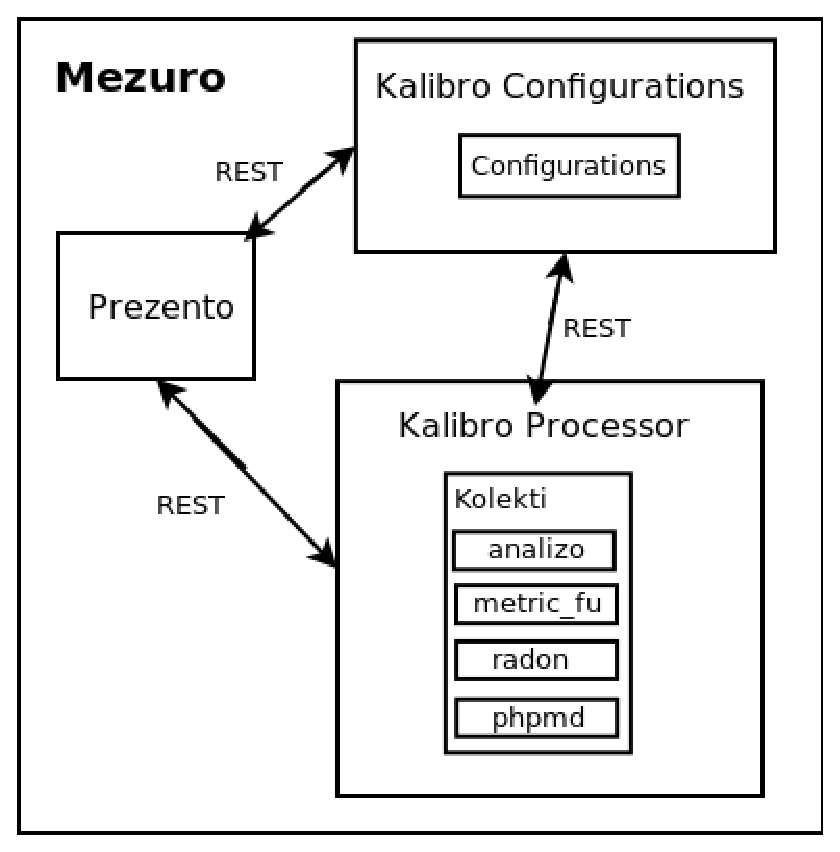
\includegraphics[keepaspectratio=true,scale=0.5]
    {figuras/mezuro_arch_v2.eps}
  \caption{Arquitetura do Mezuro}
	\label{fig:mezuro_arch_v2}
\end{figure}

\newpage

Onde os serviços são:

\begin{itemize}
  \item \textit{Prezento}\footnote{\url{https://github.com/mezuro/prezento}}:
        para a interface gráfica do usuário;
  \item \textit{Kalibro Processor}\footnote{\url{https://github.com/mezuro/kalibro\_processor}}:
        para a análise do código;
  \item \textit{Kalibro Configurations}\footnote{\url{https://github.com/mezuro/kalibro\_configurations}}:
        para o gerenciamento das configurações.
\end{itemize}

A decisão de dividir o Kalibro em serviços separados foi tomada para deixar
cada um deles com menos responsabilidades, facilitando a manutenção e evolução
\cite{camarinhaOSS2015}. E a comunicação entre estes serviços é feita através
do Kalibro Client\footnote{\url{https://github.com/mezuro/kalibro\_client}}:
um quarto software também escrito em Ruby, mantendo a escolha de centralização
em uma única tecnologia. E, como demonstra Figura \ref{fig:mezuro_arch_v2},
para simplificar a implementação, também foi decidido que a comunicação entre
os serviços seria RESTful.

O outro elemento presente na imagem, chamado \textbf{Kolekti}\footnote{\url{https://github.com/mezuro/kolekti}},
é uma \textit{Rubygem} responsável pela extração e abstração dos coletores
(Analizo, MetricFu, Radon, PHPMD), o que resulta em um \textit{parse} para o
\textit{Kalibro Processor} tornando fácil a adição de novos coletores no Mezuro.
Cada \textit{kolekti} possui o seu respectivo repositório na organização no
Github: kolekti\_analizo\footnote{\url{https://github.com/mezuro/kolekti\_analizo}},
kolekti\_metricfu\footnote{\url{https://github.com/mezuro/kolekti\_metricfu}},
kolekti\_radon\footnote{\url{https://github.com/mezuro/kolekti\_radon}} e
kolekti\_cc\_phpmd\footnote{\url{https://github.com/mezuro/kolekti\_cc\_phpmd}}.

Outro componente desenvolvido pela equipe do Mezuro, é o \textbf{Likeno}. A
função principal dele é conectar serviços através de uma API RESTful. Parte do
é extraído do \textit{Kalibro Client}, porém simplificando e estabelecendo uma
prática de reuso para projetos que não tenham relação com Mezuro. O
\textit{Likeno} também foi empacotado como uma \textit{Gem} e é similar à outras
APIs, como a \textit{ActiveResource}\footnote{\url{https://github.com/rails/activeresource}}
e a \textit{her}\footnote{\url{https://github.com/remiprev/her}}.

Dada essa arquitetura baseada em serviços, as principais funcionalidades podem
ser divididas em dois grupos:

\begin{itemize}
  \item Projeto
    \begin{itemize}
    \item \textit{Download} do código-fonte a partir de repositórios (Git,
    Subversion, Bazaar etc) ou via arquivo compactado;
        \item Escolha da periodicidade do processamento do código (1 dia, 2 dias,
        semanal, quinzenal e mensal);
        \item Escolha de qual configuração de métricas cada repositório irá
        utilizar;
        \item Nota de cada métrica da configuração para cada arquivo do
        repositório;
        \item Análise gráfica de cada arquivo do repositório por meio de um
        gráfico de pontos com notas ao longo do tempo;
        \item Resultados públicos e acessíveis à comunidade.
    \end{itemize}
    \item Configuração
    \begin{itemize}
    \item Criação de configuração e a possibilidade de clonagem;
        \item Estatísticas sobre as configurações mais populares dentro da
        comunidade;
        \item Criação de intervalos qualitativos associados aos valores das
        métricas;
        \item Criação de grupos de leitura para a interpretação textual dos
        resultados das métricas;
        \item Combinações de métricas nativas para criação de análises compostas
        e mais complexas.''
    \end{itemize}
\end{itemize}

Com esse conjunto de funcionalidades, o Mezuro apresenta-se como uma ferramenta
inovadora. Neste trabalho, destaca-se, portanto, que o Mezuro é uma ferramenta
com grande potencial, e funcionalidades inovadoras e úteis. A arquitetura
modularizada gera uma abordagem de interpretação adequada par ao monitoramento
das métricas. Por isso, o foco deste trabalho é melhorar a camada de interface
\textit{Web} de interação com o usuário, para exatamente aproveitar/alavancar este
potencial.

\section{Mezuro: Prezento}

O Prezento é a camada da interface \textit{Web} do
Mezuro. Desenvolvido em Ruby on Rails, atualmente utiliza as versões 2.3.0 do
Ruby e 4.2.4 do Rails. Versões estas que estão em constante mudança, pois os
mantenedores têm como intuito usufruir o que há de mais recente das funcionalidades
dessa tecnologia. Esta será a principal camada trabalhada neste trabalho de
conclusão de curso, pois é nela que há a interação com o usuário.

Ela está disponível em dois idiomas: português e inglês. Quase todas as rotas
do site são acessíveis publicamente, sem necessidade de inscrição na plataforma.
Porém, Caso o usuário queira criar Configurações de Métrica, Grupos de Leitura,
e/ou adicionar projetos para a avaliação é necessário realizar o cadastro.

Ao acessar a página inicial\footnote{\url{http://mezuro.org/}}, é exposto ao
usuário uma breve explicação sobre a plataforma. No menu superior fixo, estão
presentes as opções: Início, Projetos, Repositórios, Configurações, Grupos de
Leitura, Entrar, Inscrever-se e um \textit{dropdown menu} com a escolha do
Idioma. Próximo ao rodapé da página, são exibidos os últimos cinco projetos,
repositórios e configurações criadas. A Figura \ref{fig:mezuro-homepage}
mostra a página inicial.

\begin{figure}[!htb]
	\centering
    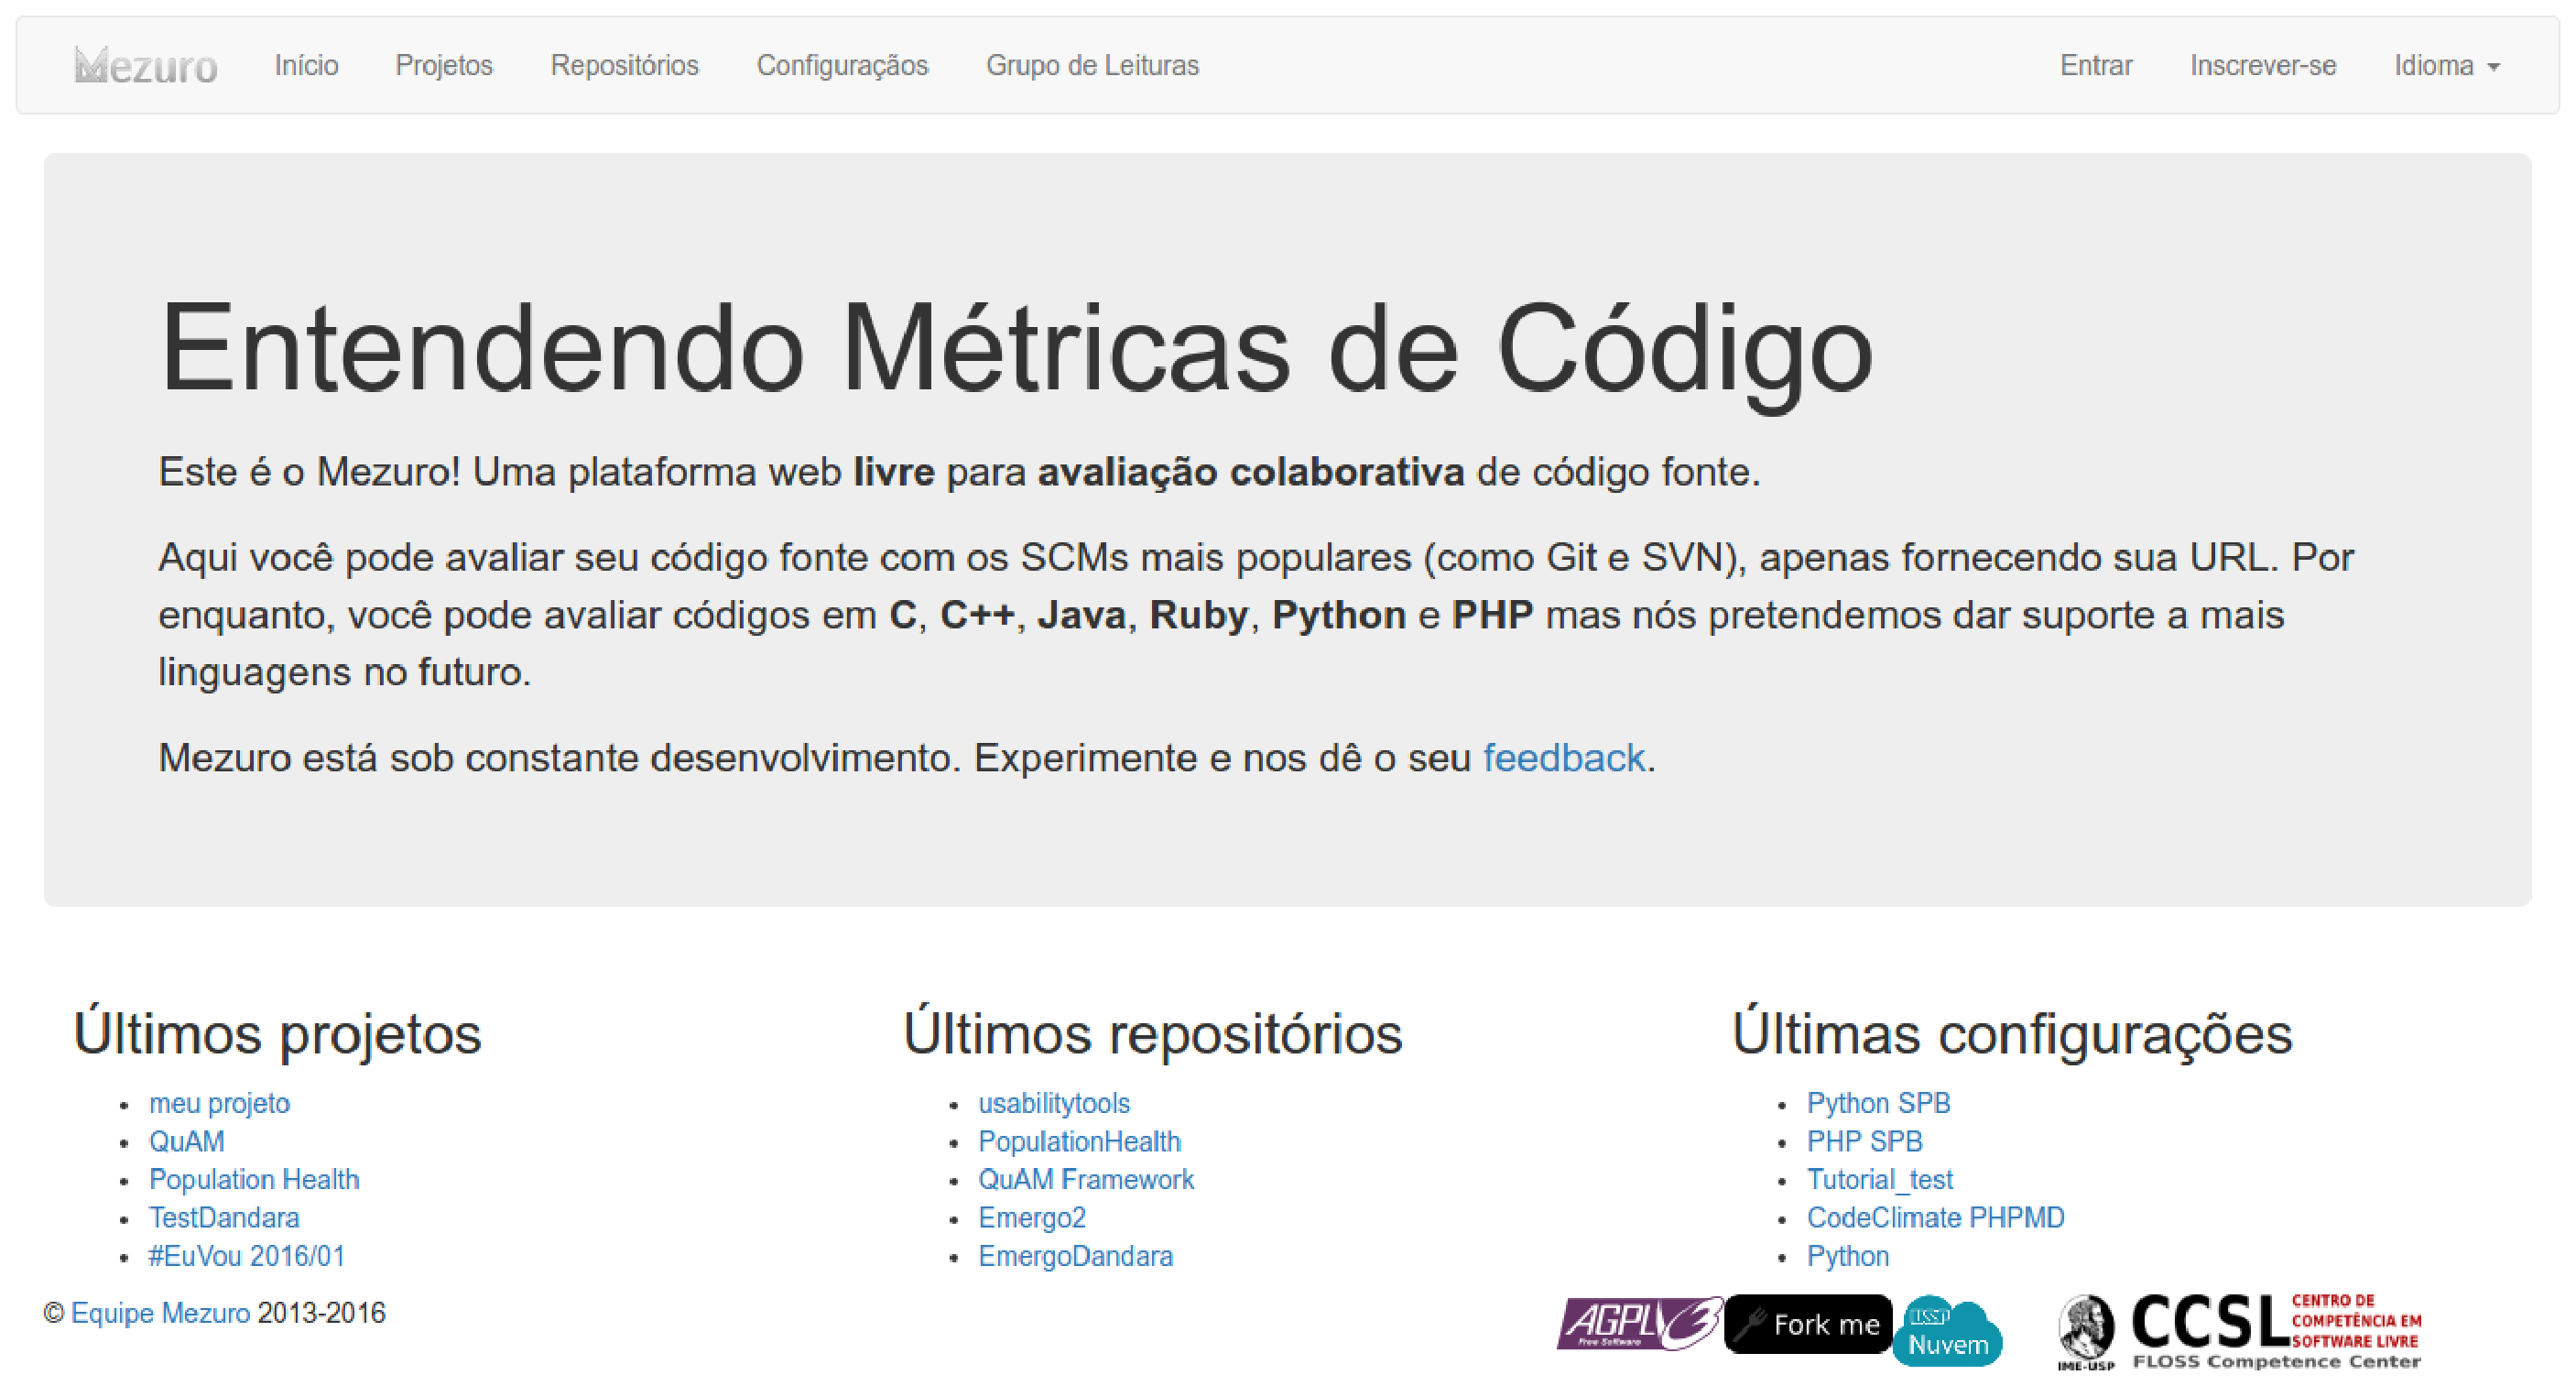
\includegraphics[keepaspectratio=true,scale=0.3]
    {figuras/mezuro-homepage.eps}
  \caption{Mezuro - Página Inicial}
	\label{fig:mezuro-homepage}
\end{figure}

\newpage

Para realizar o cadastro de usuário, basta informar nome, e-mail e senha. E o
e-mail fica sendo utilizado como identificador de acesso.

\begin{figure}[!htb]
	\centering
    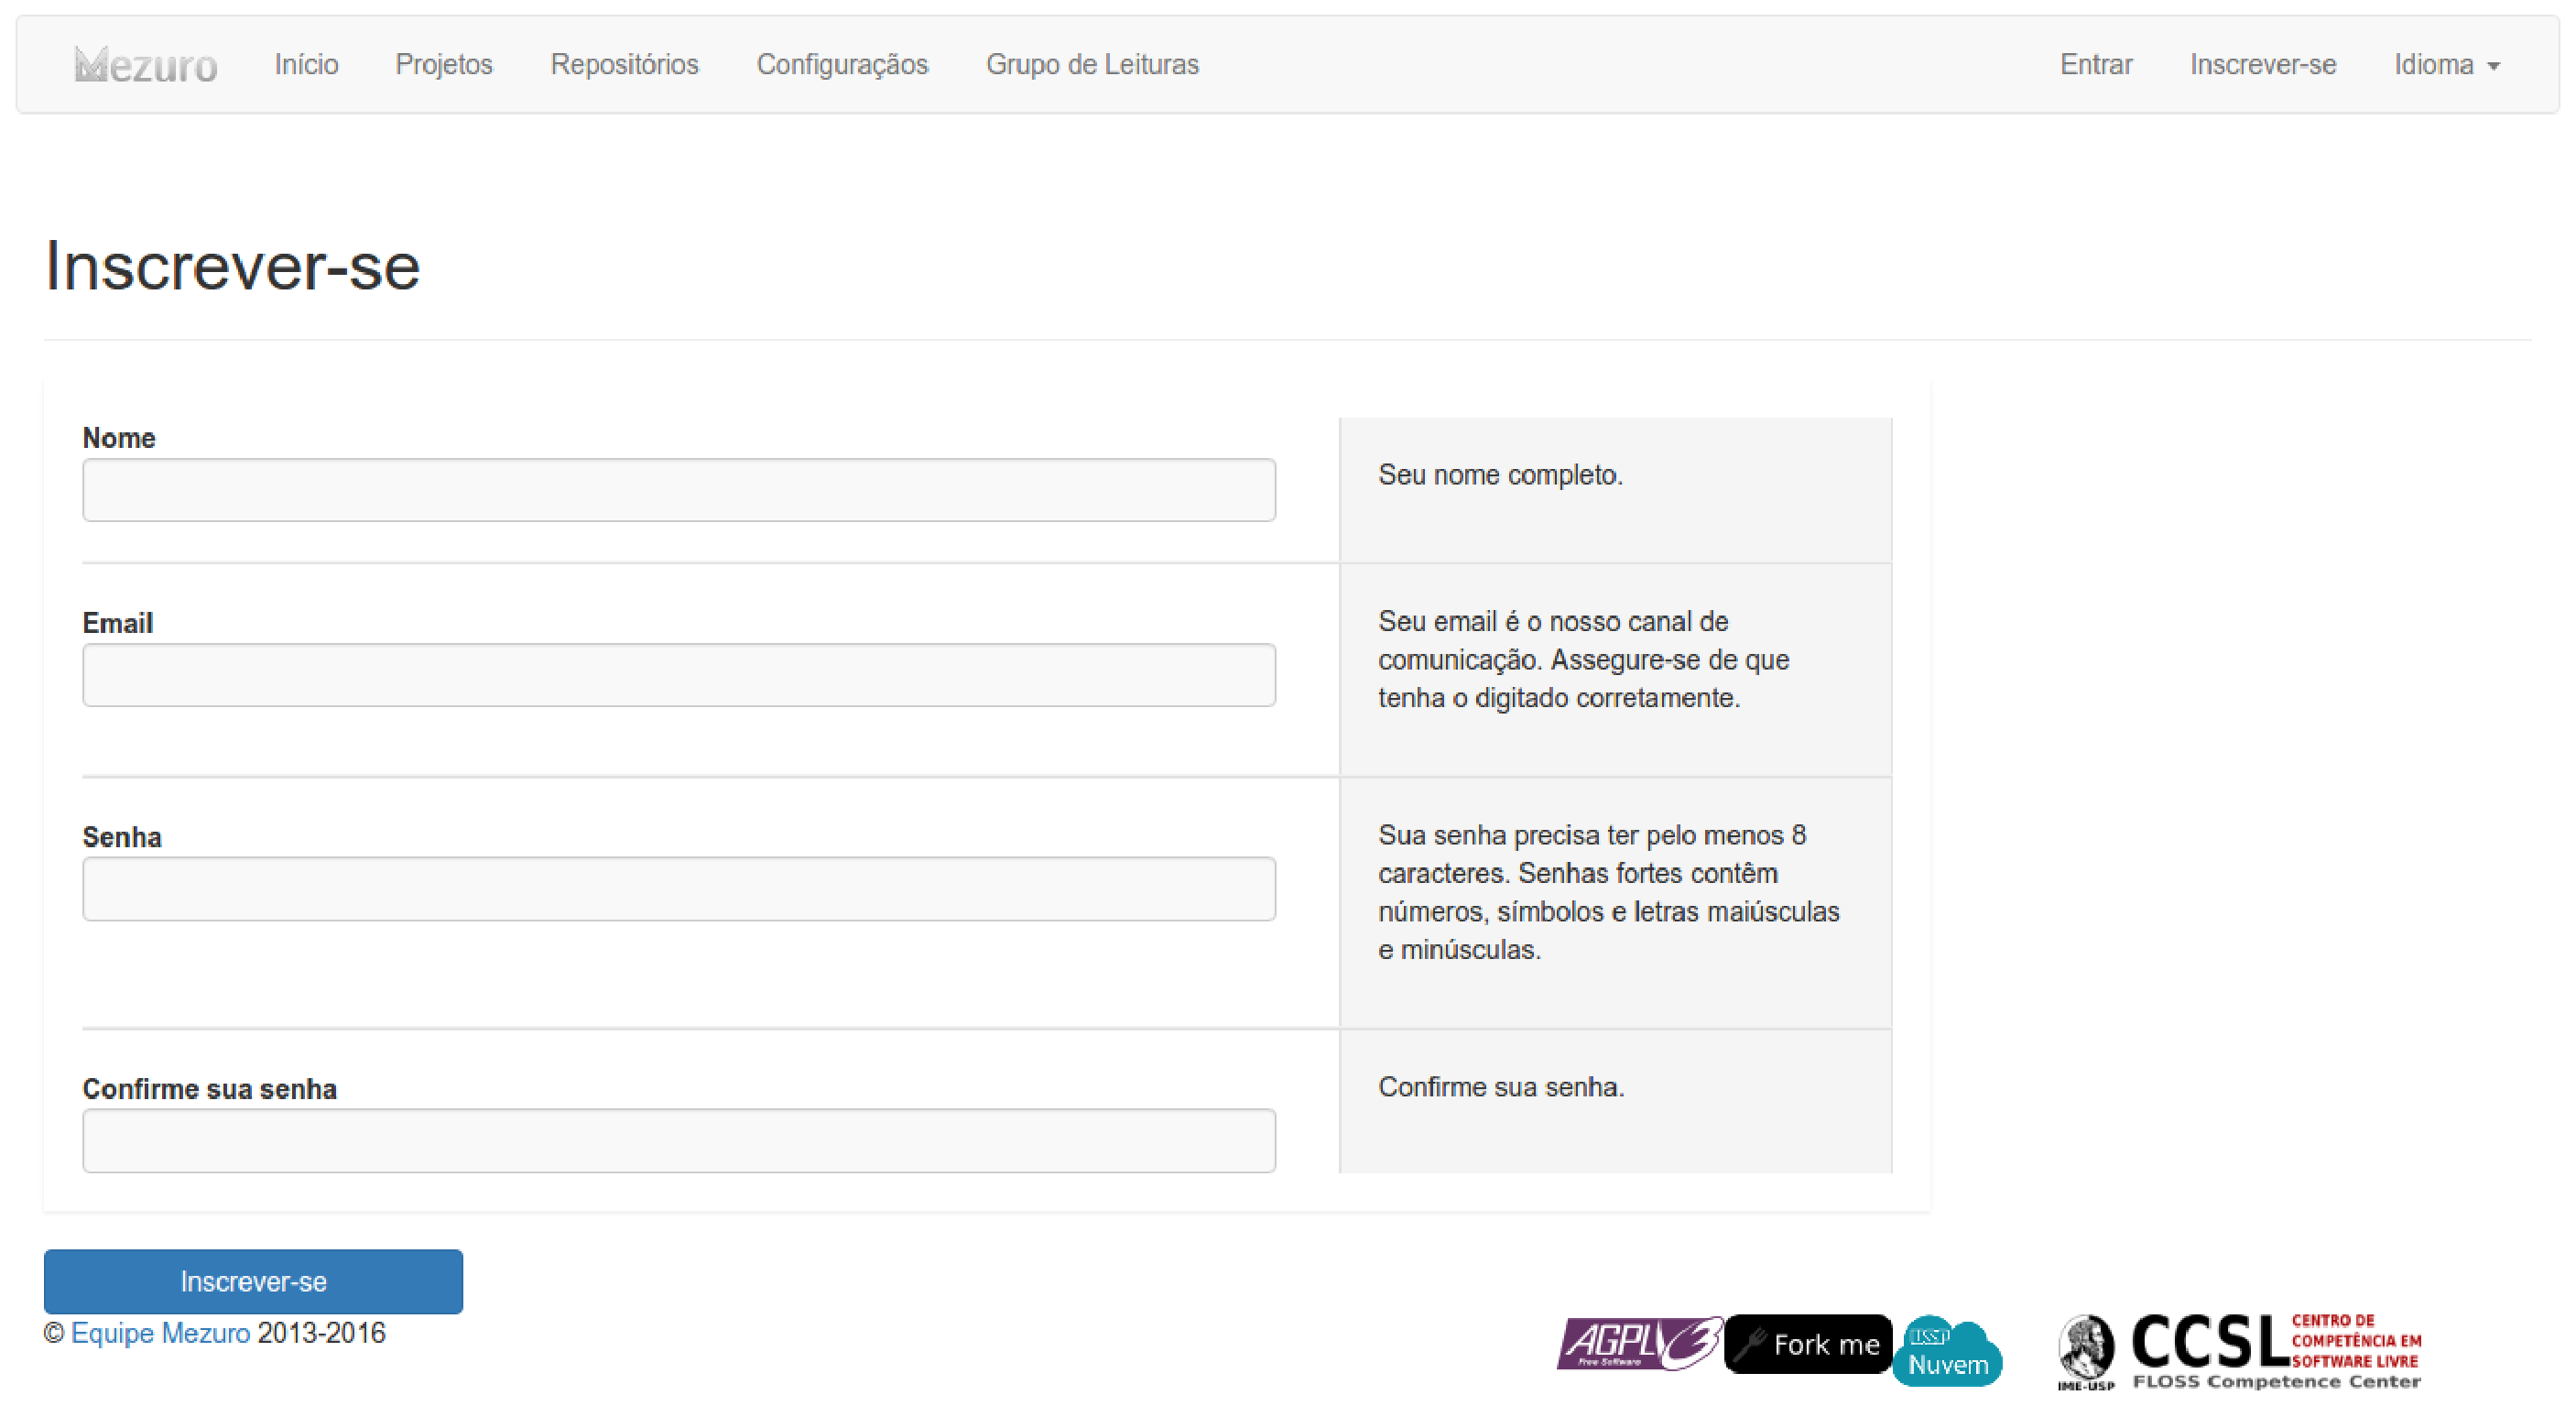
\includegraphics[keepaspectratio=true,scale=0.3]
    {figuras/mezuro-cadastro.eps}
  \caption{Mezuro - Página Cadastro de Usuário}
	\label{fig:mezuro-cadastro}
\end{figure}

\newpage

Na página destinada à exibição dos projetos, uma lista semelhante à Figura
\ref{fig:mezuro-projetos-v2} é mostrada. Se o usuário for o dono projeto, além do
botão \textbf{Mostrar}, é acrescido o botão \textbf{Editar}. Caso contrário, o
único acesso é o de visualização do projeto. Para criar um projeto, basta
informar o nome, descrição e (caso queira) a Url de alguma imagem relacionada.
Ao visualizar o projeto, o usuário pode conferir os repositórios adicionados.

\begin{figure}[!htb]
	\centering
    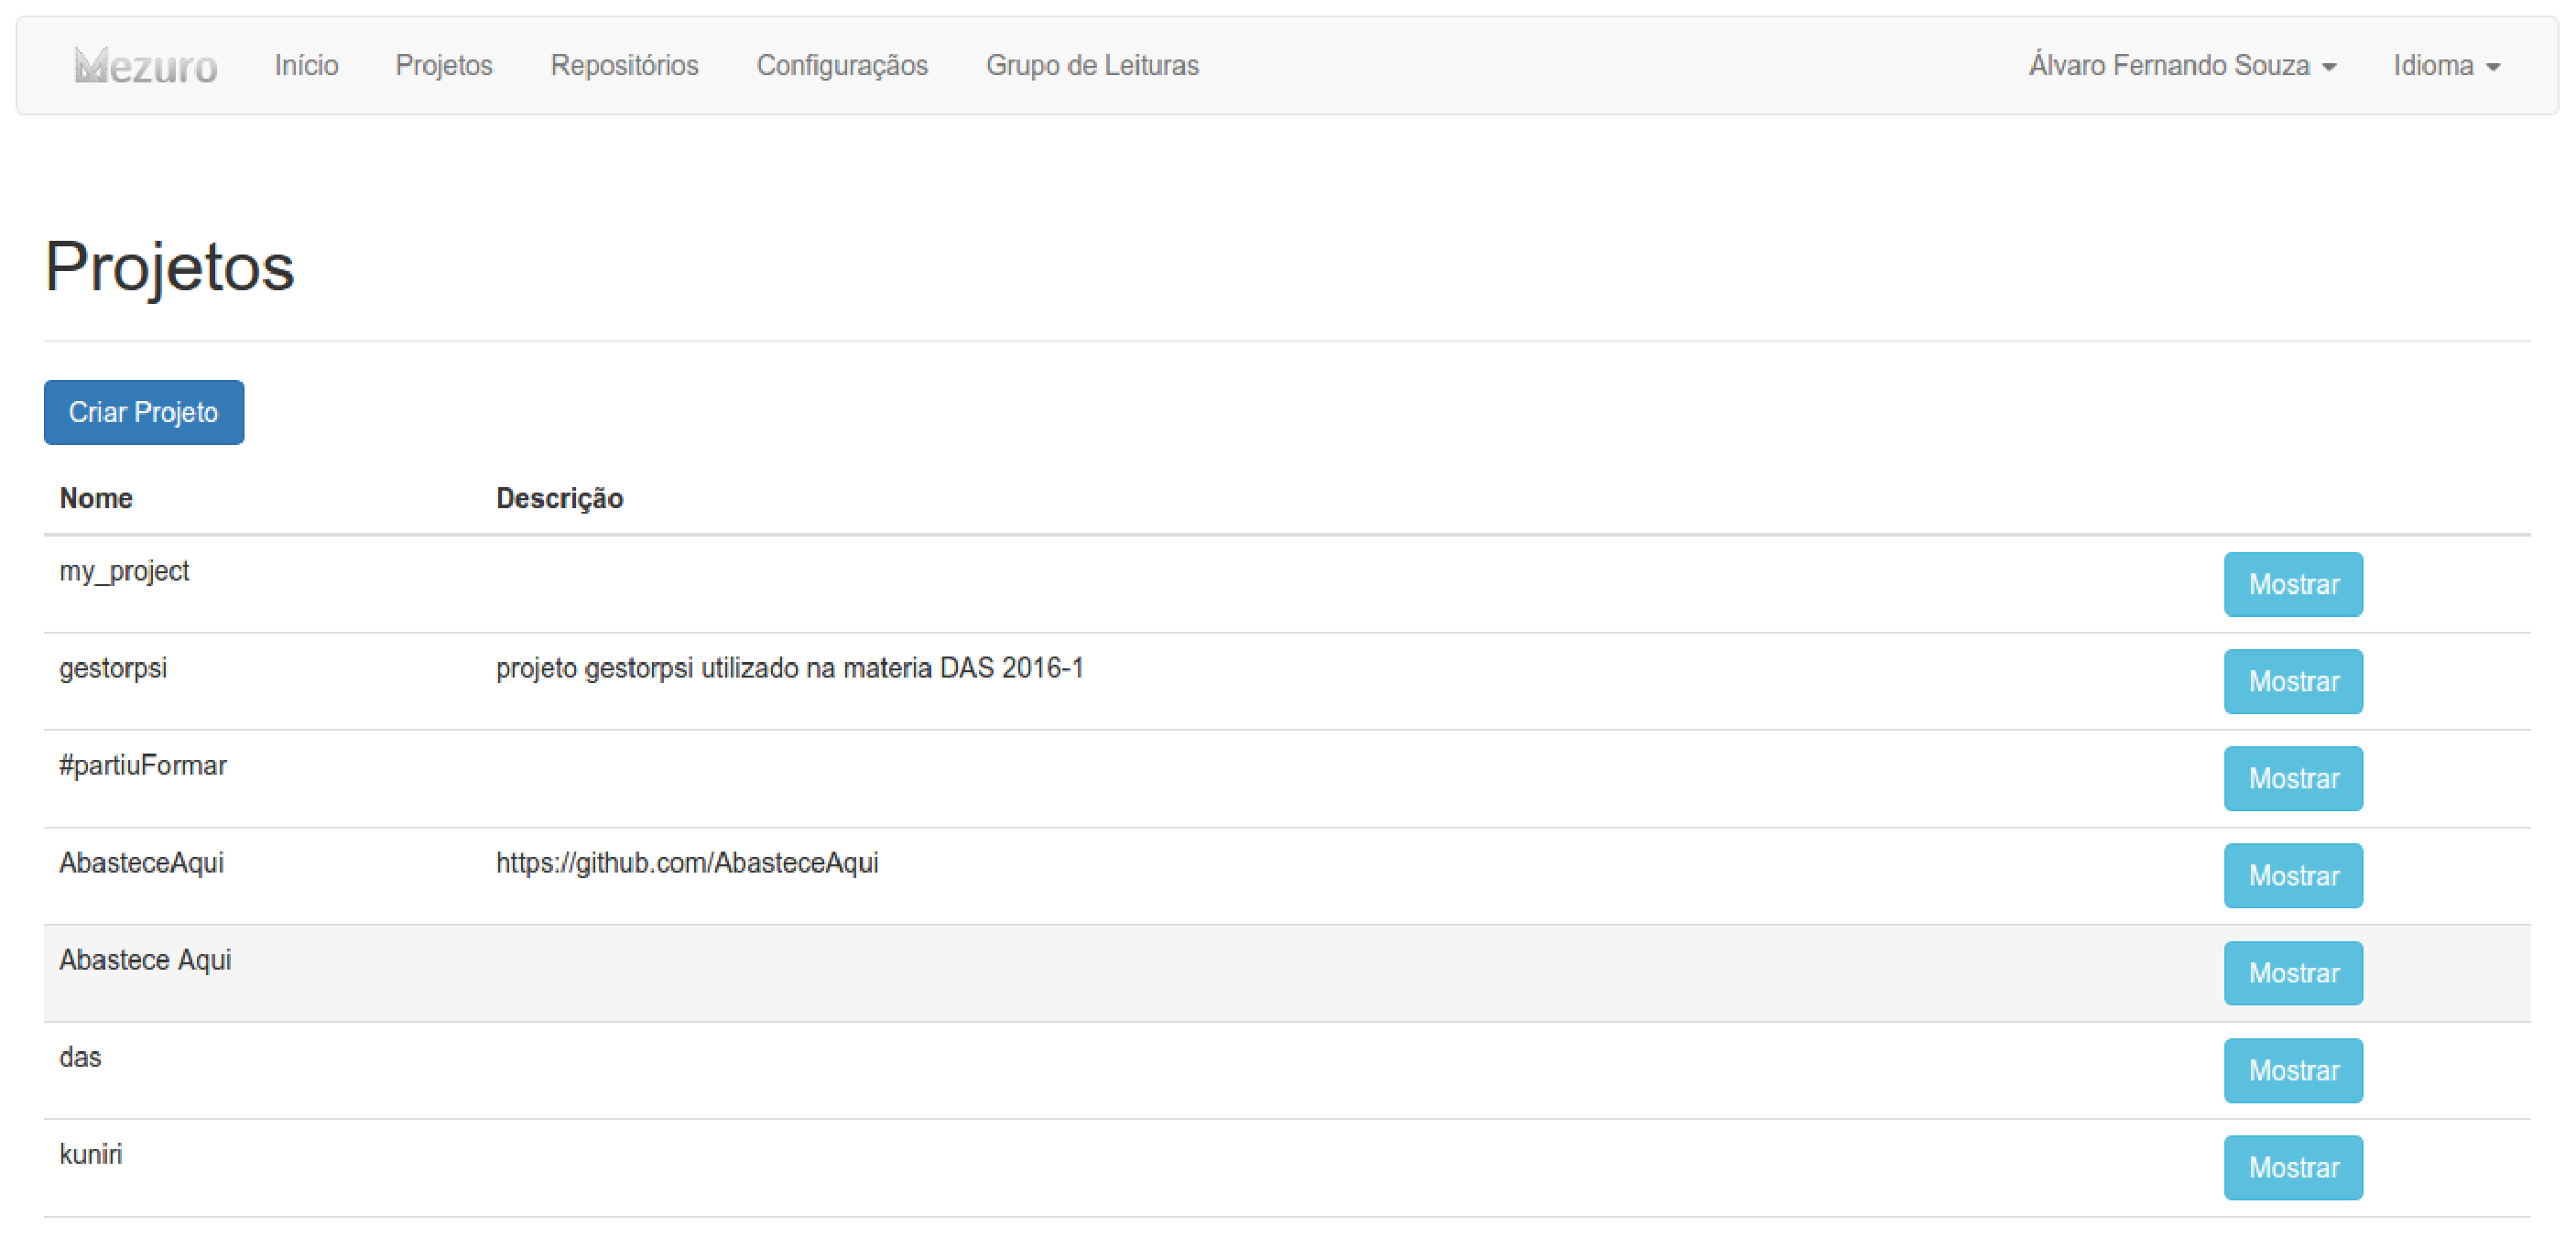
\includegraphics[keepaspectratio=true,scale=0.3]
    {figuras/mezuro-projetos-v2.eps}
  \caption{Mezuro - Lista de Projetos}
	\label{fig:mezuro-projetos-v2}
\end{figure}

\begin{figure}[!htb]
	\centering
    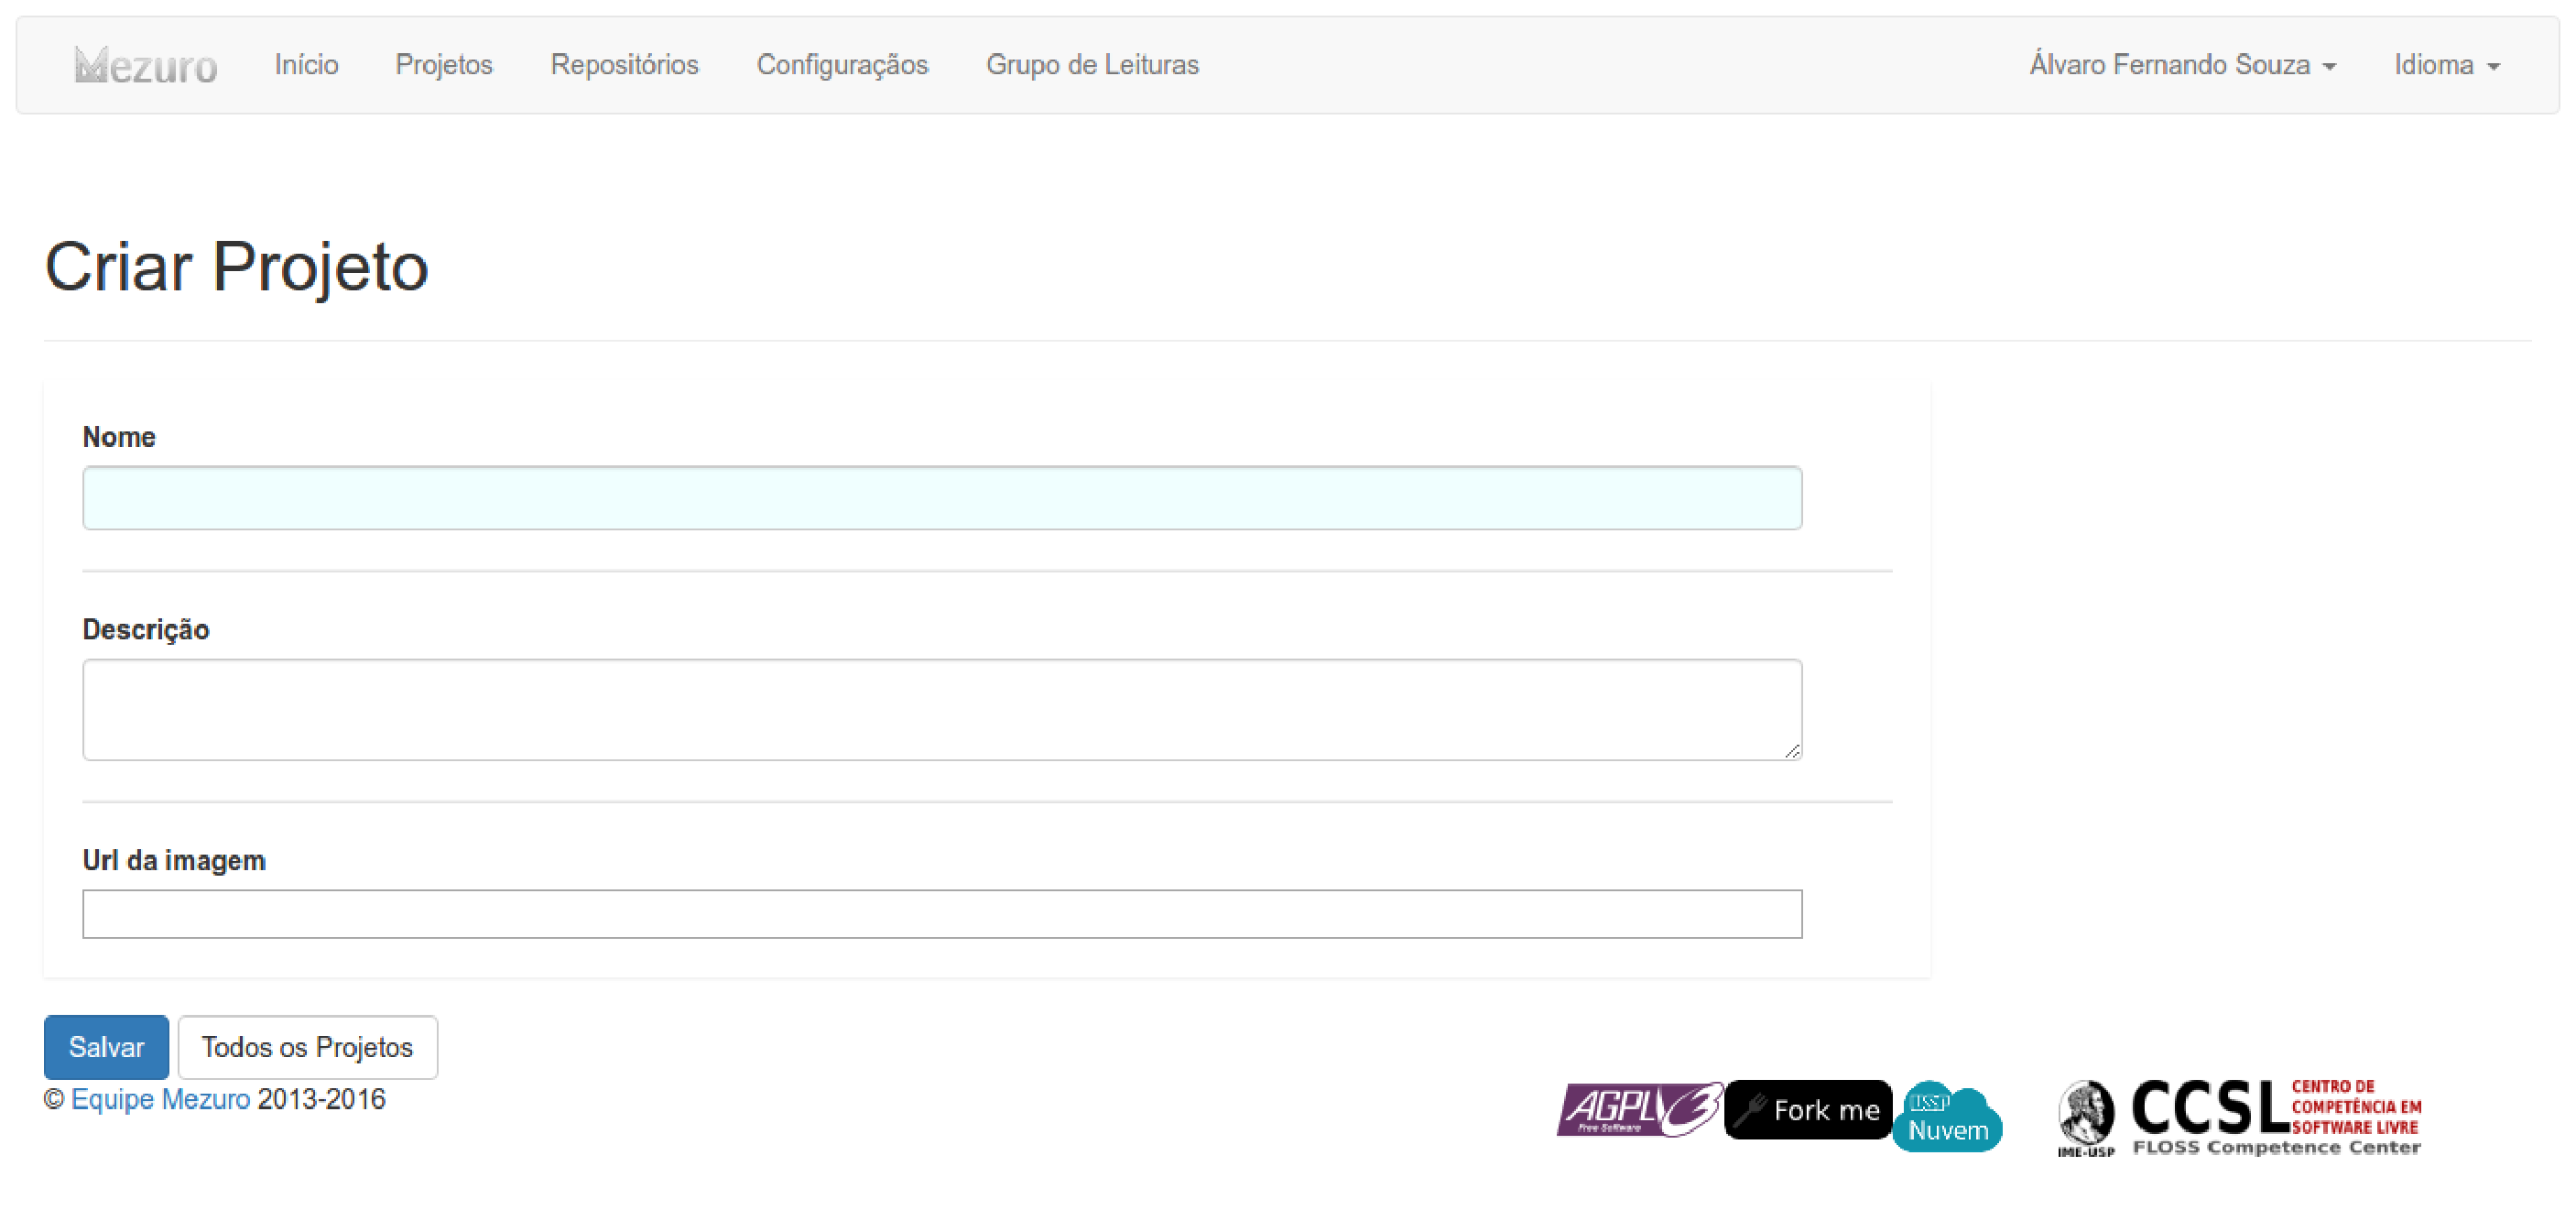
\includegraphics[keepaspectratio=true,scale=0.3]
    {figuras/mezuro-projeto-cadastro.eps}
  \caption{Mezuro - Cadastro de Projetos}
	\label{fig:mezuro-projeto-cadastro}
\end{figure}

\newpage

\begin{figure}[!htb]
	\centering
    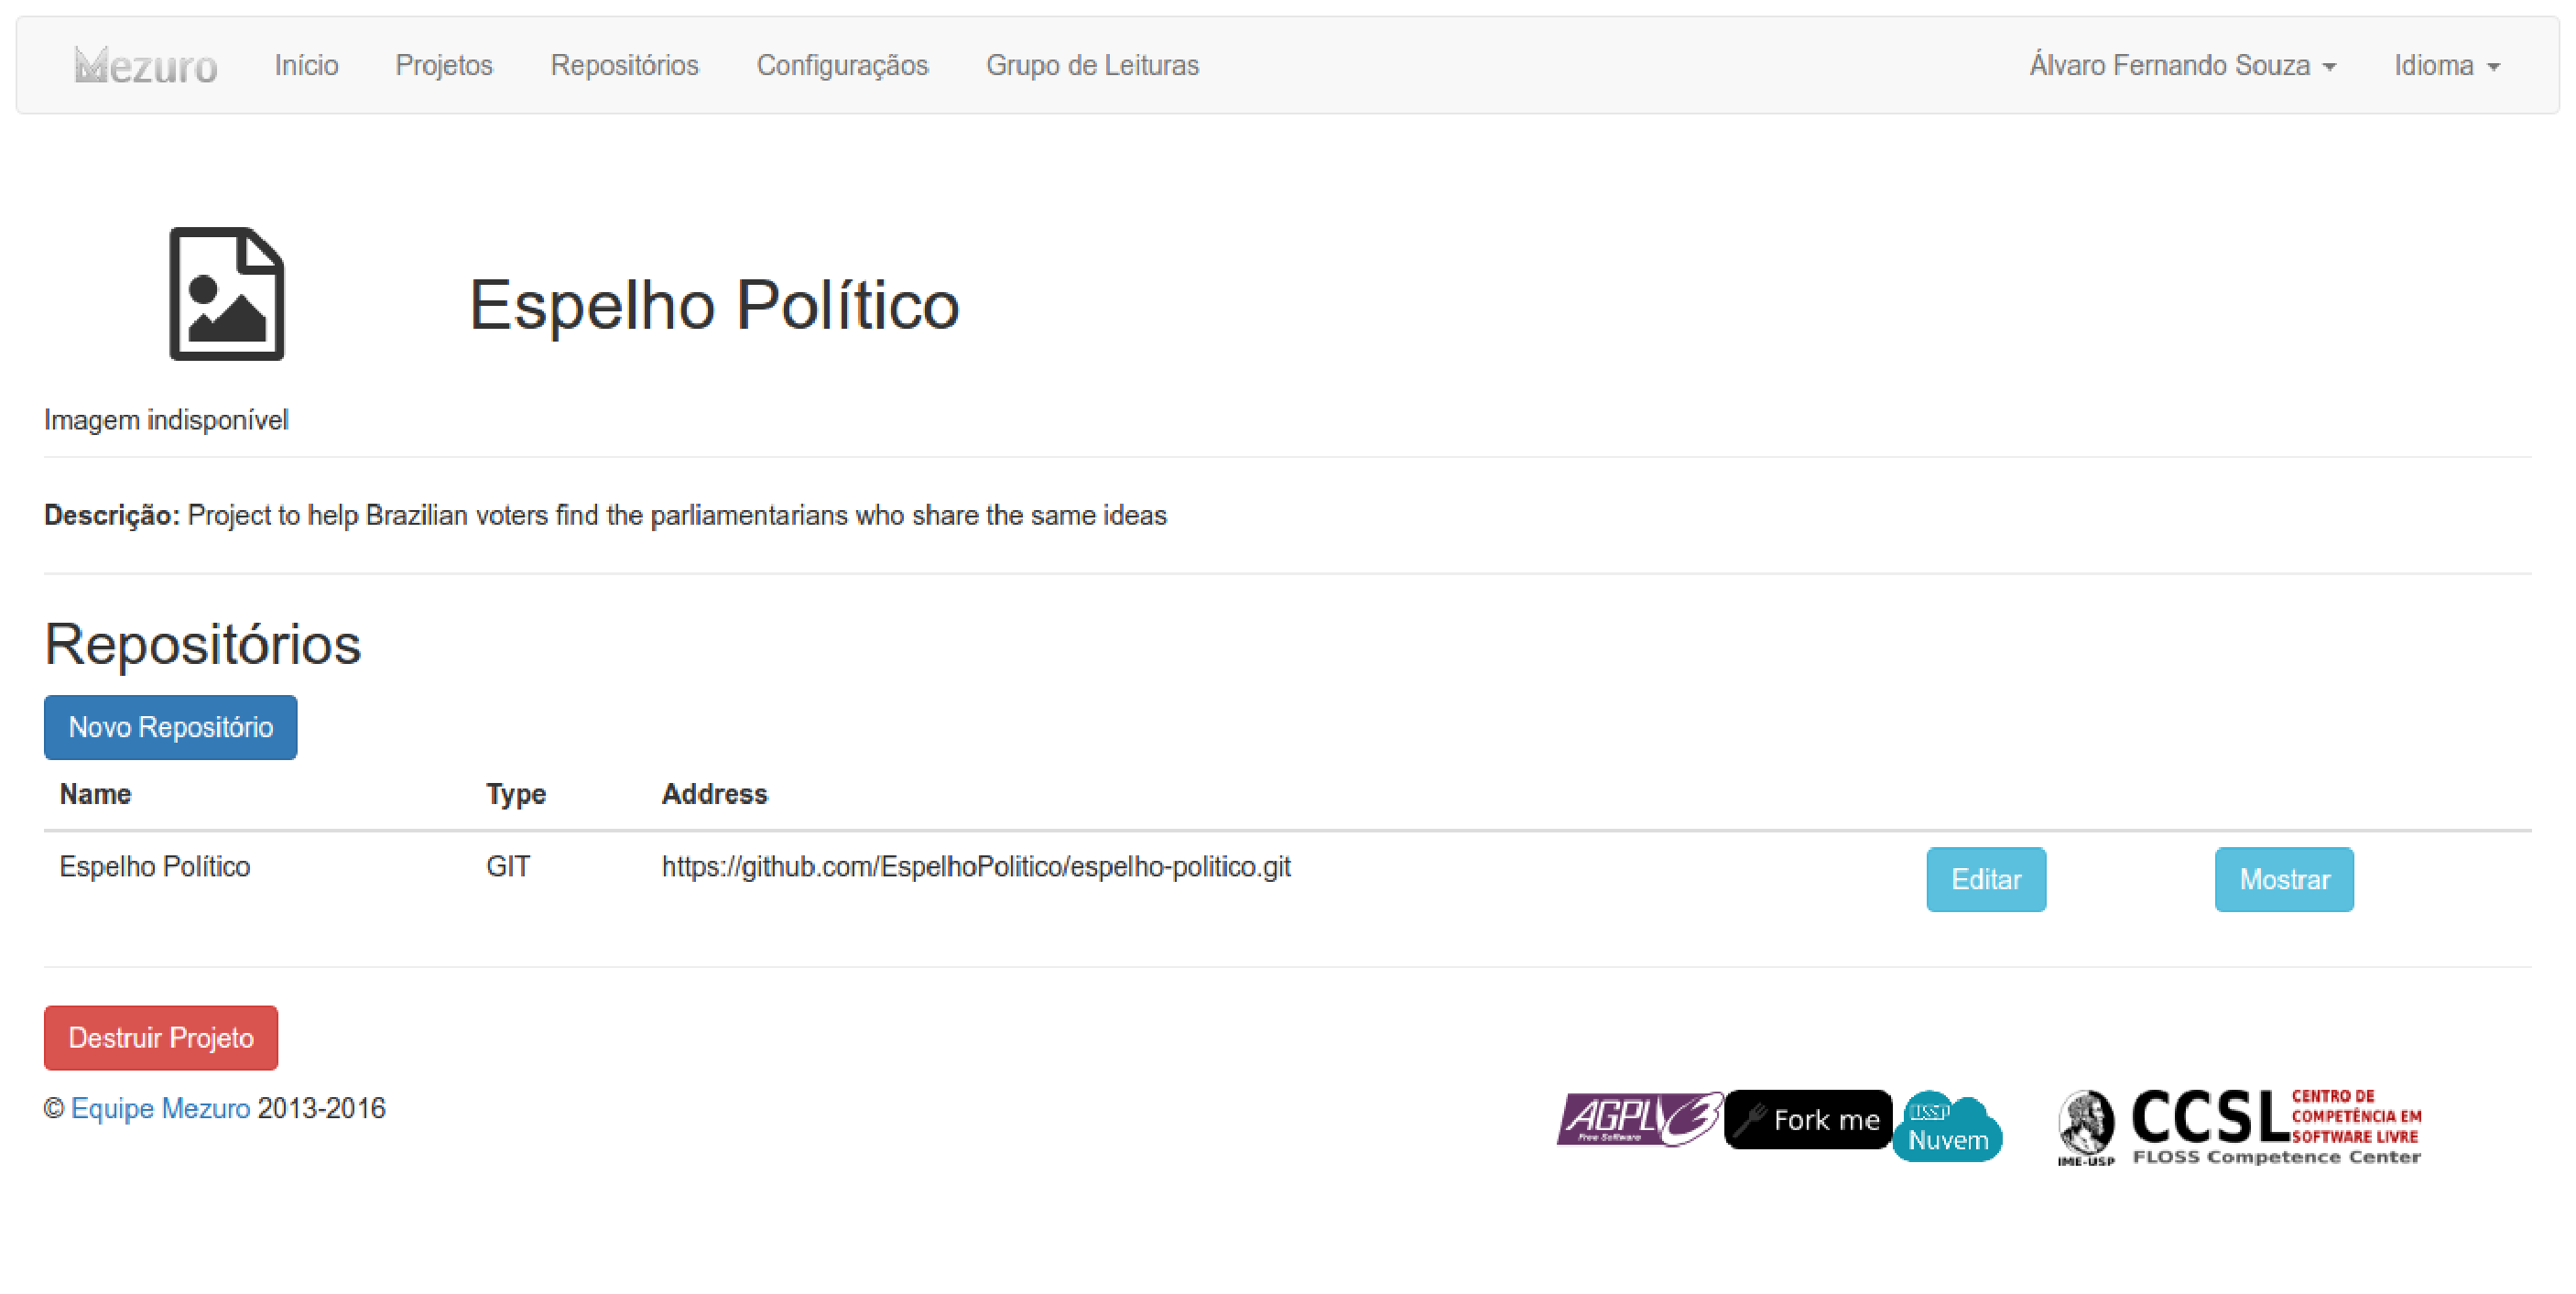
\includegraphics[keepaspectratio=true,scale=0.3]
    {figuras/mezuro-projeto-view.eps}
  \caption{Mezuro - Página de Projeto}
	\label{fig:mezuro-projeto-view}
\end{figure}

\newpage

A lista de repositórios tem um comportamento semelhante à de projetos, vide
Figura \ref{fig:mezuro-repositorios-v2}. Na criação de um repositório, é
necessário informar: nome, descrição, licença, tipo de sistema de
versionamento, endereço acessível para o repositório de código, qual ramo
deseja-se que seja realizada a avaliação (se \textit{master},
\textit{dev}, ou \textit{prod}, por exemplo), a frequência com deseja-se que o
projeto seja reprocessado e a Configuração de Métrica.

\begin{figure}[!htb]
	\centering
    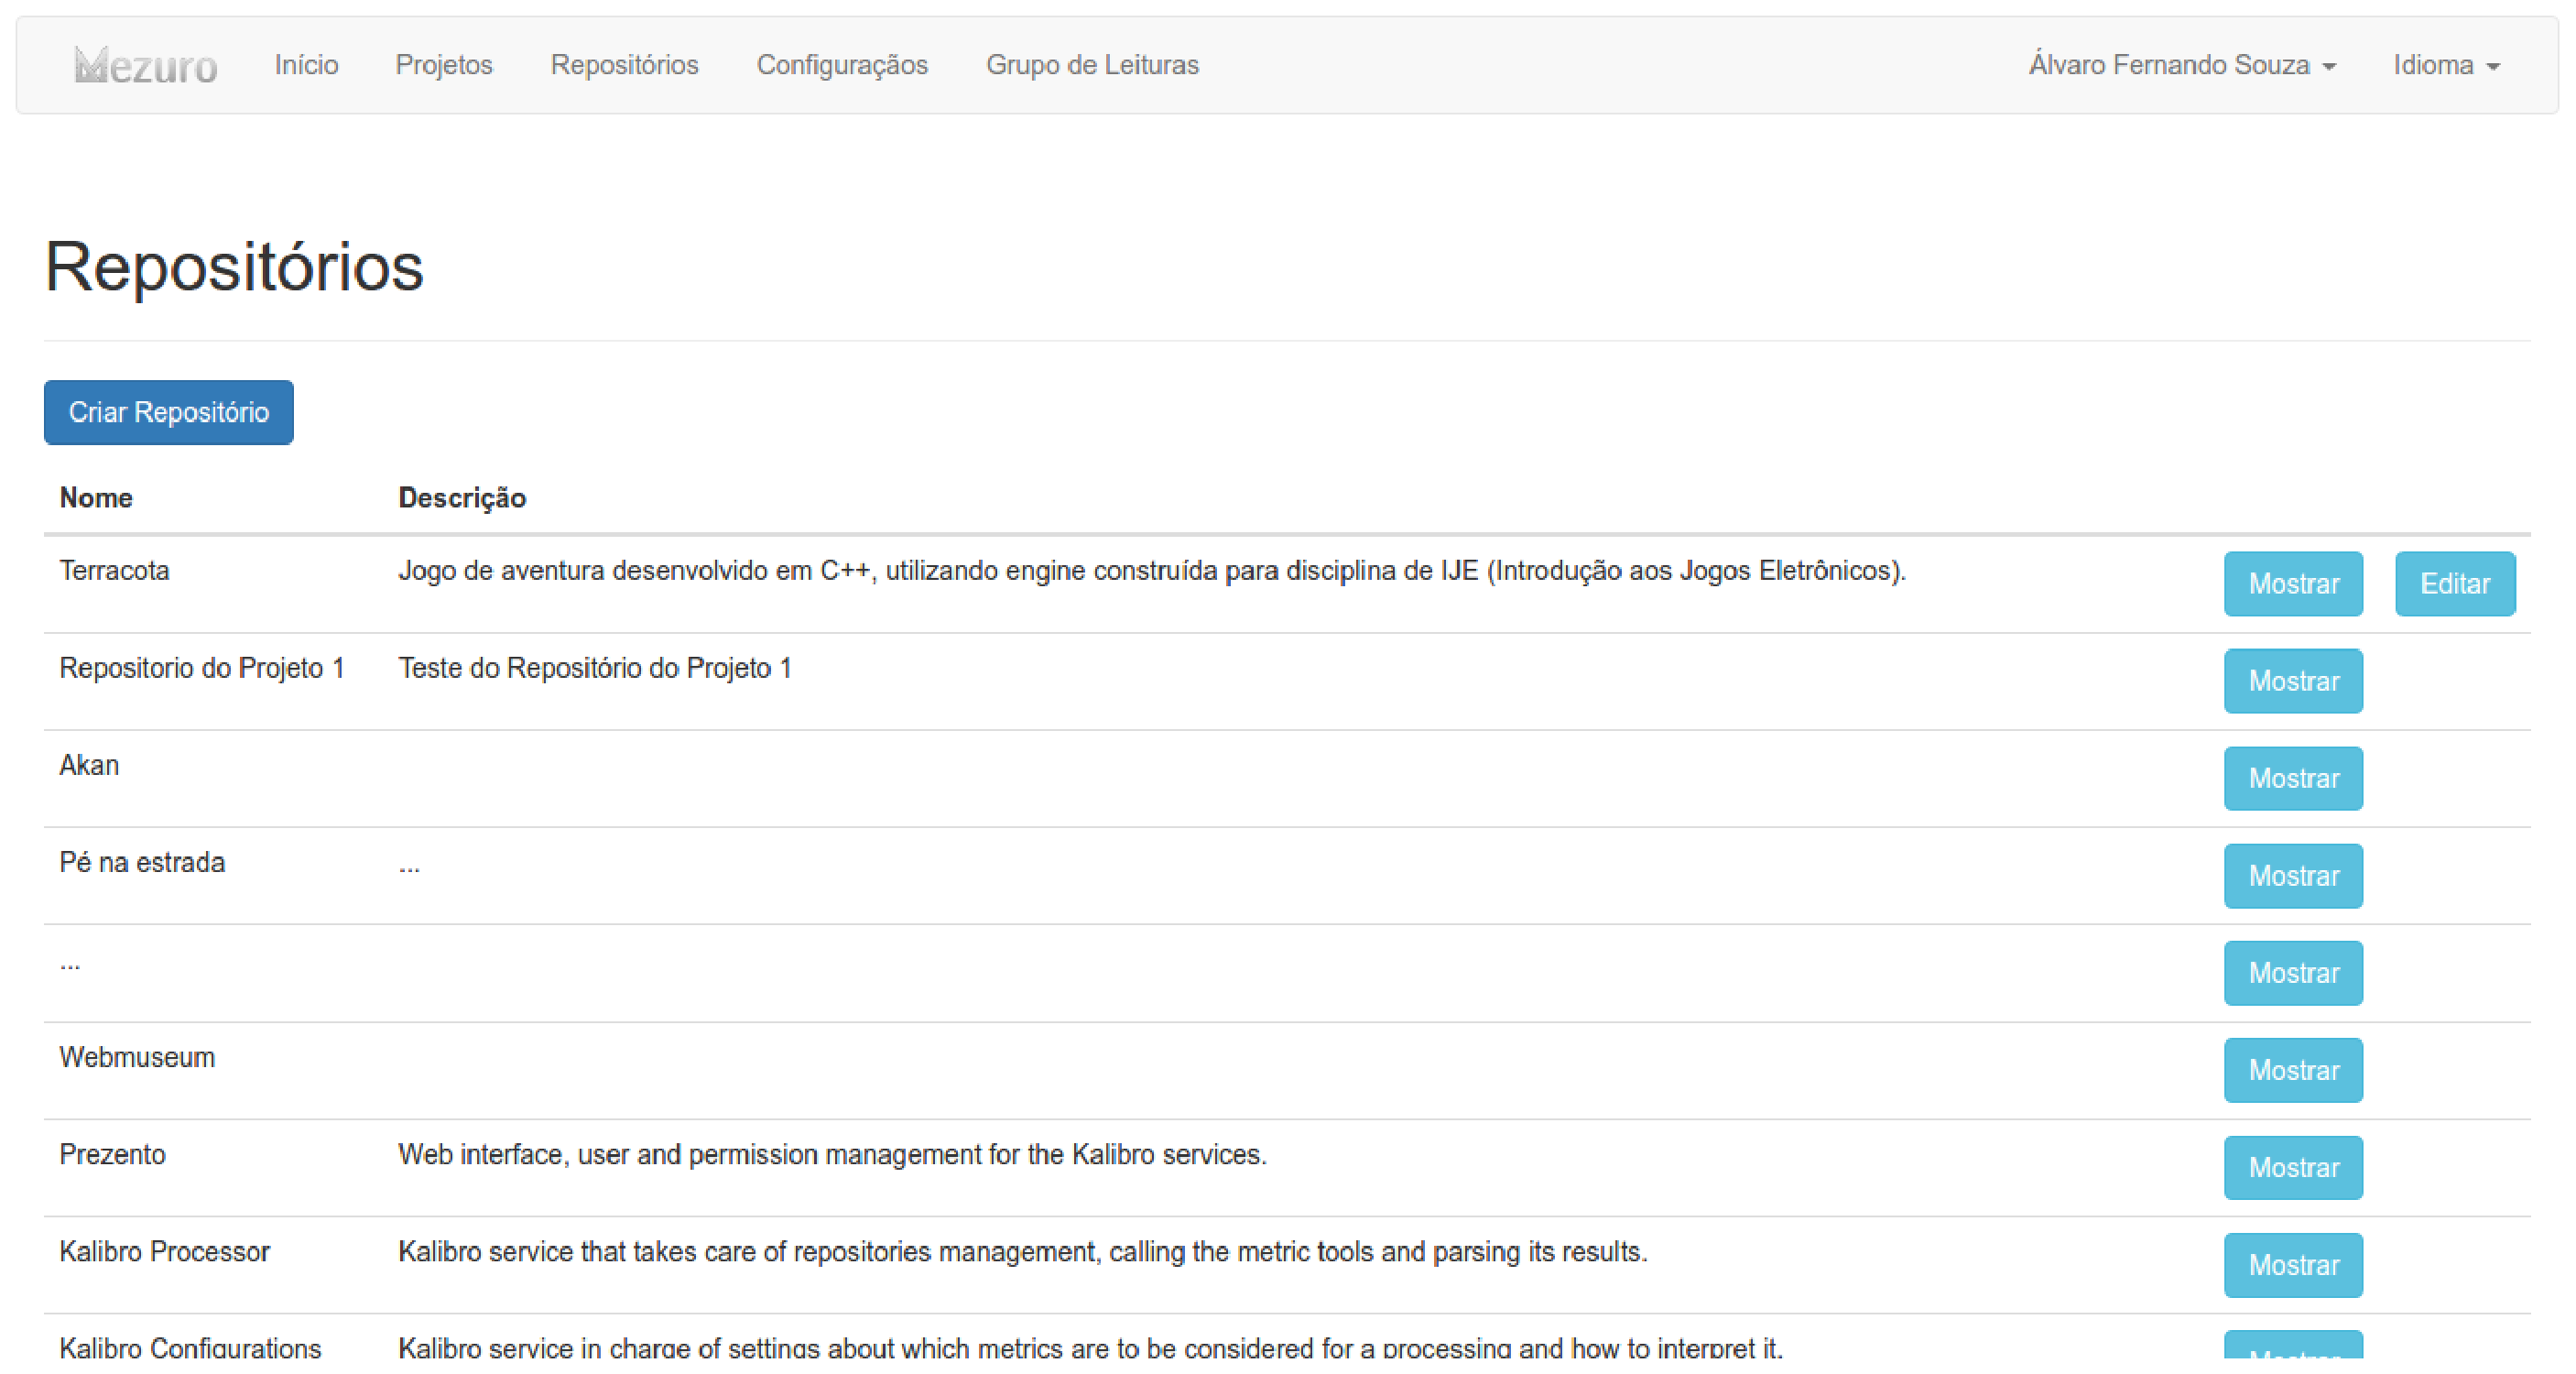
\includegraphics[keepaspectratio=true,scale=0.3]
    {figuras/mezuro-repositorios-v2.eps}
  \caption{Mezuro - Lista de Repositórios}
	\label{fig:mezuro-repositorios-v2}
\end{figure}

\newpage

\begin{figure}[!htb]
	\centering
    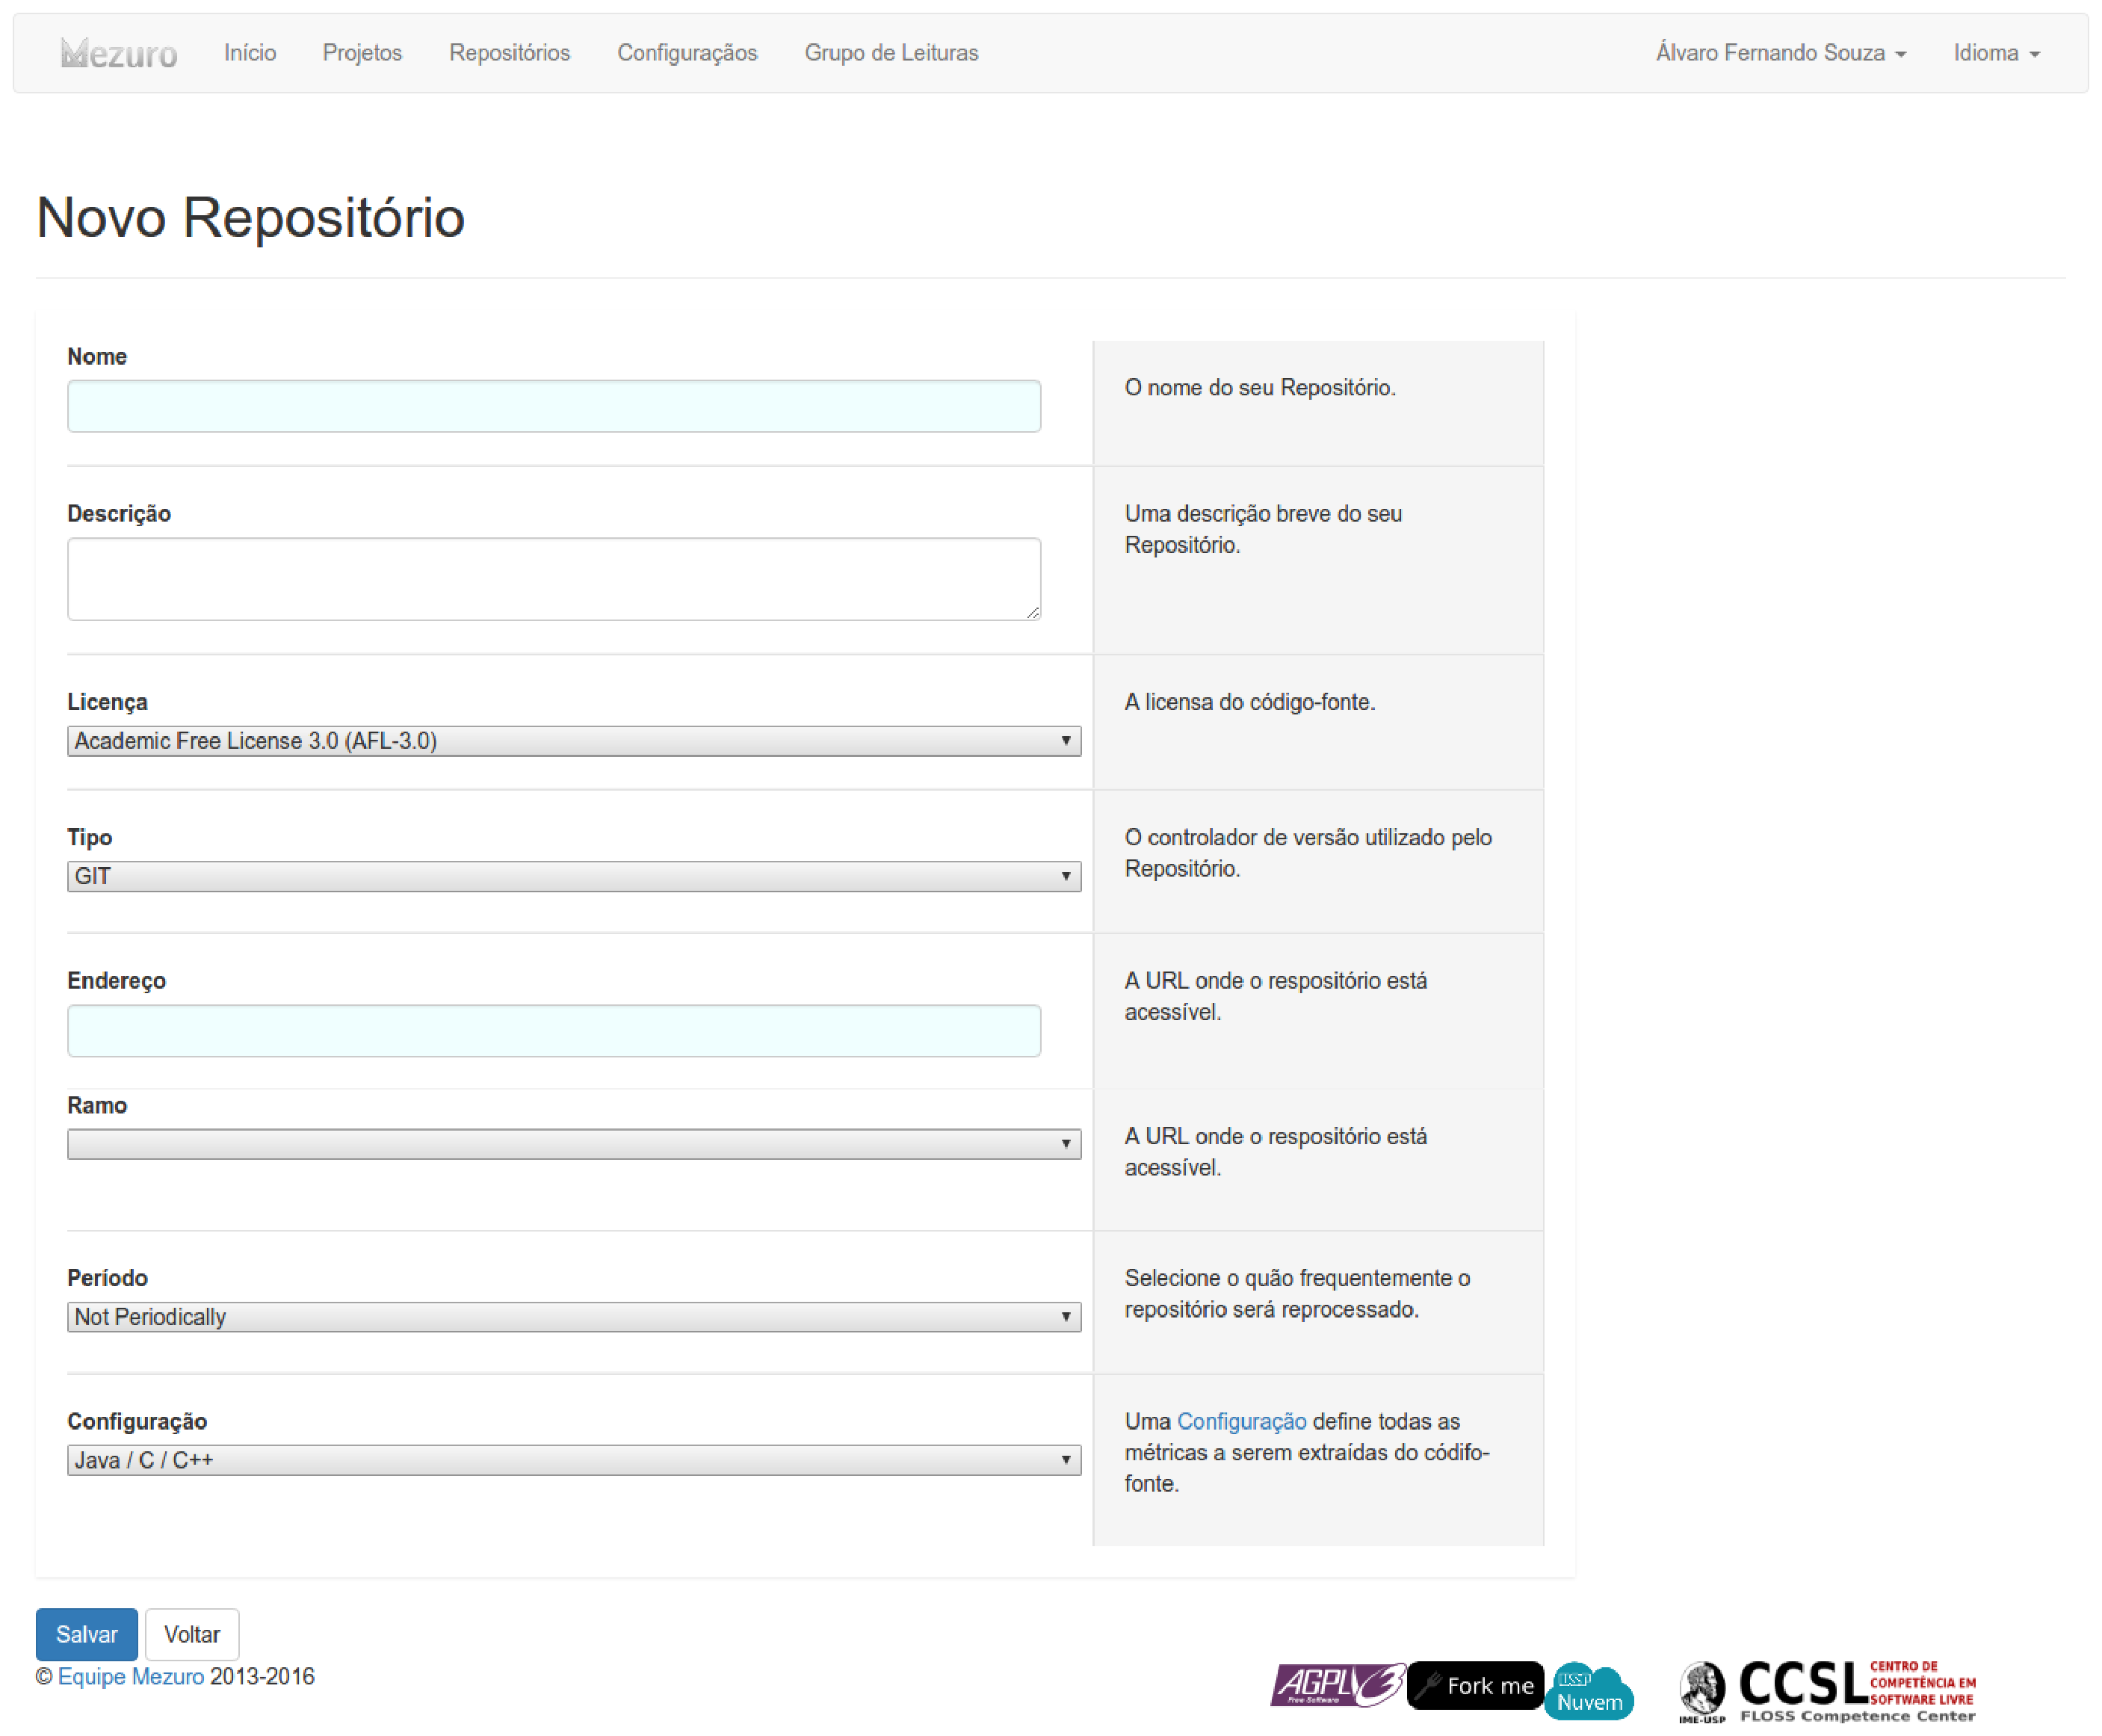
\includegraphics[keepaspectratio=true,scale=0.3]
    {figuras/mezuro-repositorio-cadastro.eps}
  \caption{Mezuro - Cadastro de Repositório}
	\label{fig:mezuro-repositorio-cadastro}
\end{figure}

\newpage

As Configurações de Métrica seguem o mesmo padrão: visualização em lista, com
botões de ``Mostrar" e ``Editar" (caso seja dono da Configuração). Para a criação
de uma nova Configuração, basta informar o Nome e a Descrição. Posteriormente, na
exibição desta Configuração criada, é possível adicionar quais métricas irão
compor esta. Na escolha da métrica, é exposto ao usuário os 4 coletores
disponíveis (Analizo, CodeClimate PHPMD, MetricFu e Radon). Escolhido a métrica,
o usuário passa então para a configuração desta métrica, informando o peso dela
para a avaliação, a forma de agregação e o grupo de leitura.

\begin{figure}[!htb]
	\centering
    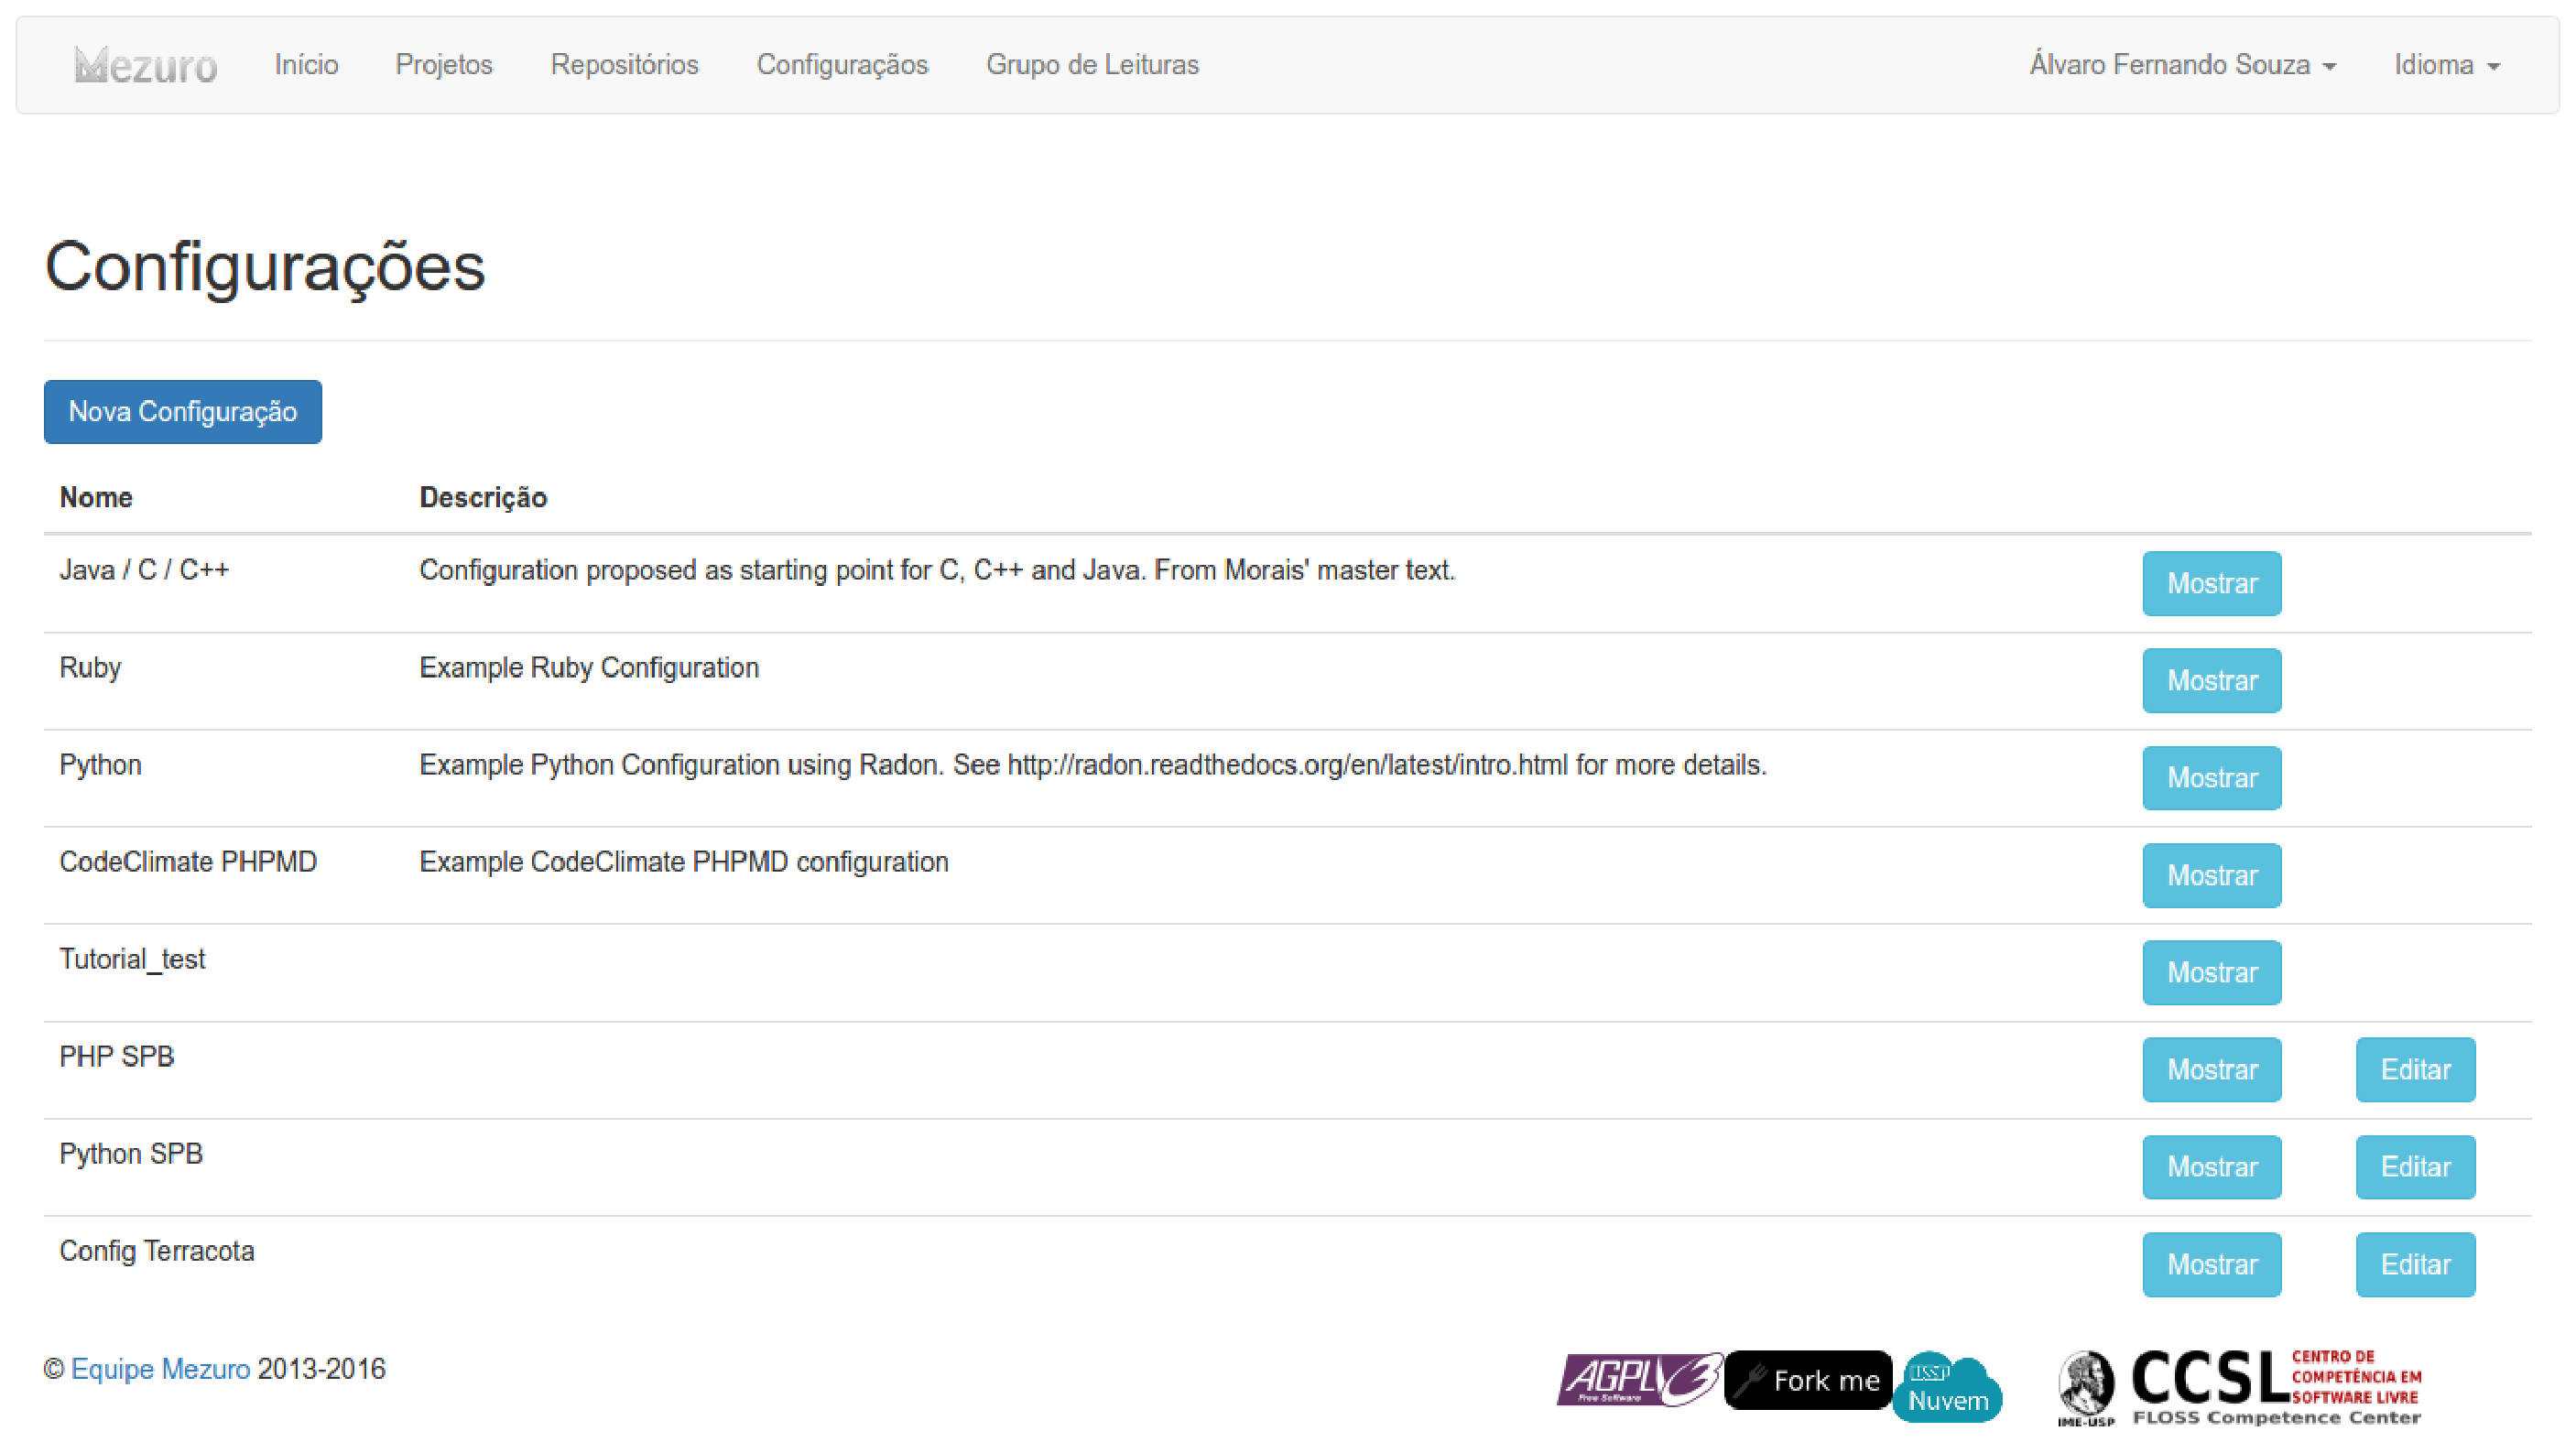
\includegraphics[keepaspectratio=true,scale=0.3]
    {figuras/mezuro-configuracoes.eps}
  \caption{Mezuro - Lista de Configurações}
	\label{fig:mezuro-configuracoes}
\end{figure}

\begin{figure}[!htb]
	\centering
    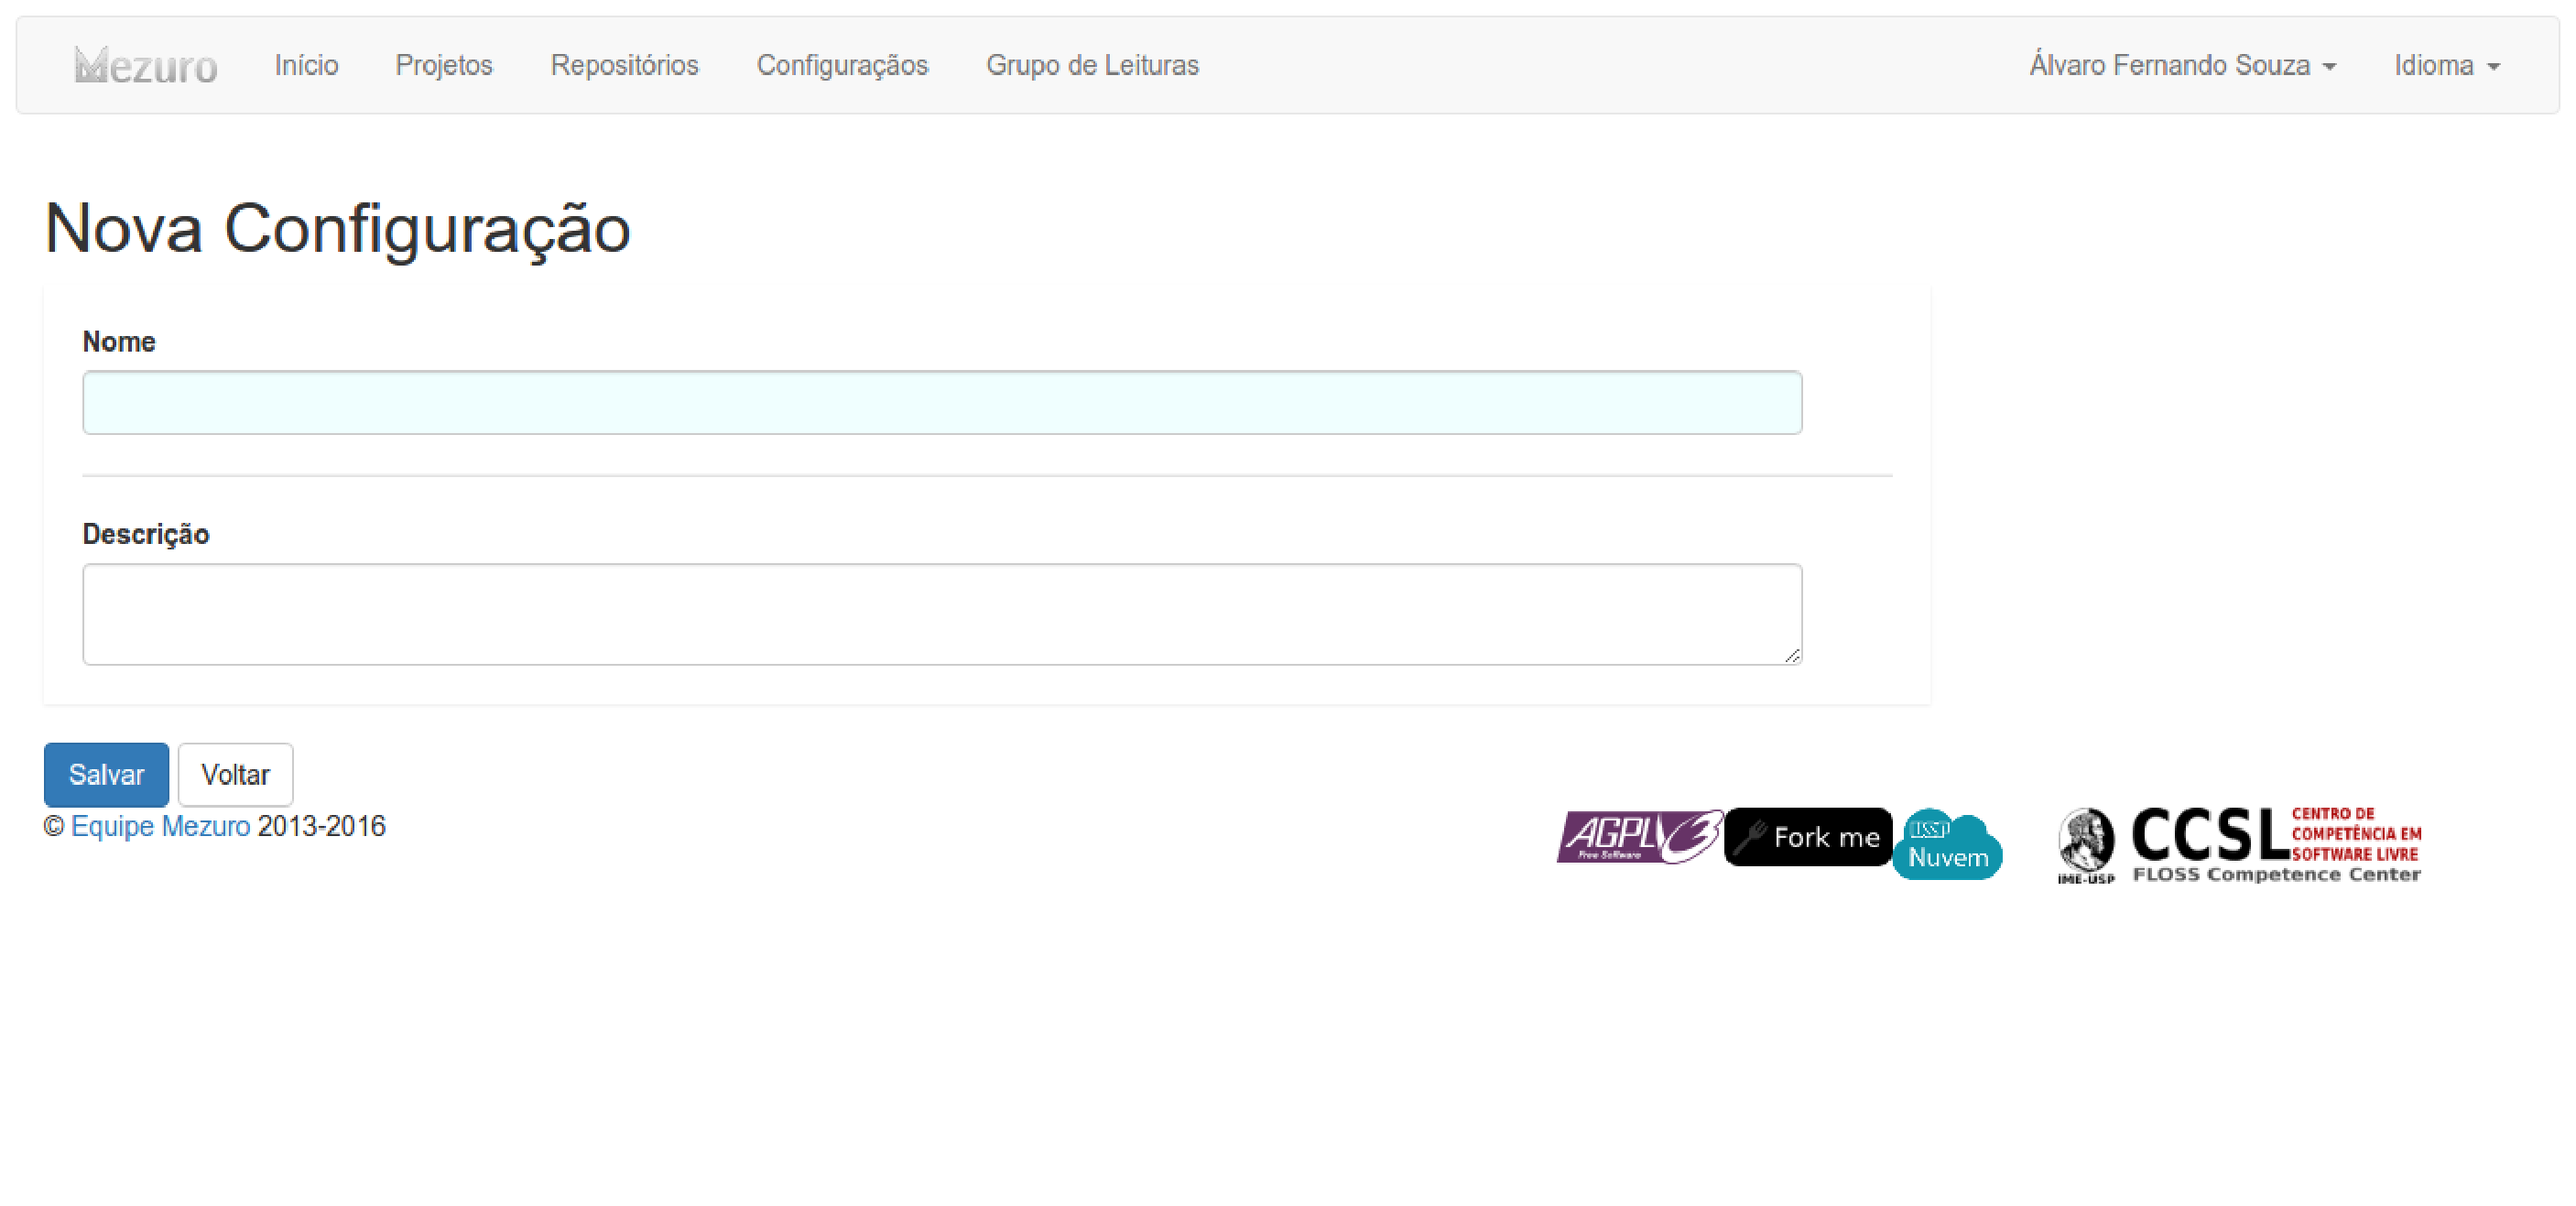
\includegraphics[keepaspectratio=true,scale=0.3]
    {figuras/mezuro-configuracao-cadastro.eps}
  \caption{Mezuro - Cadastro de Configuração}
	\label{fig:mezuro-configuracao-cadastro}
\end{figure}

\newpage

\begin{figure}[!htb]
	\centering
    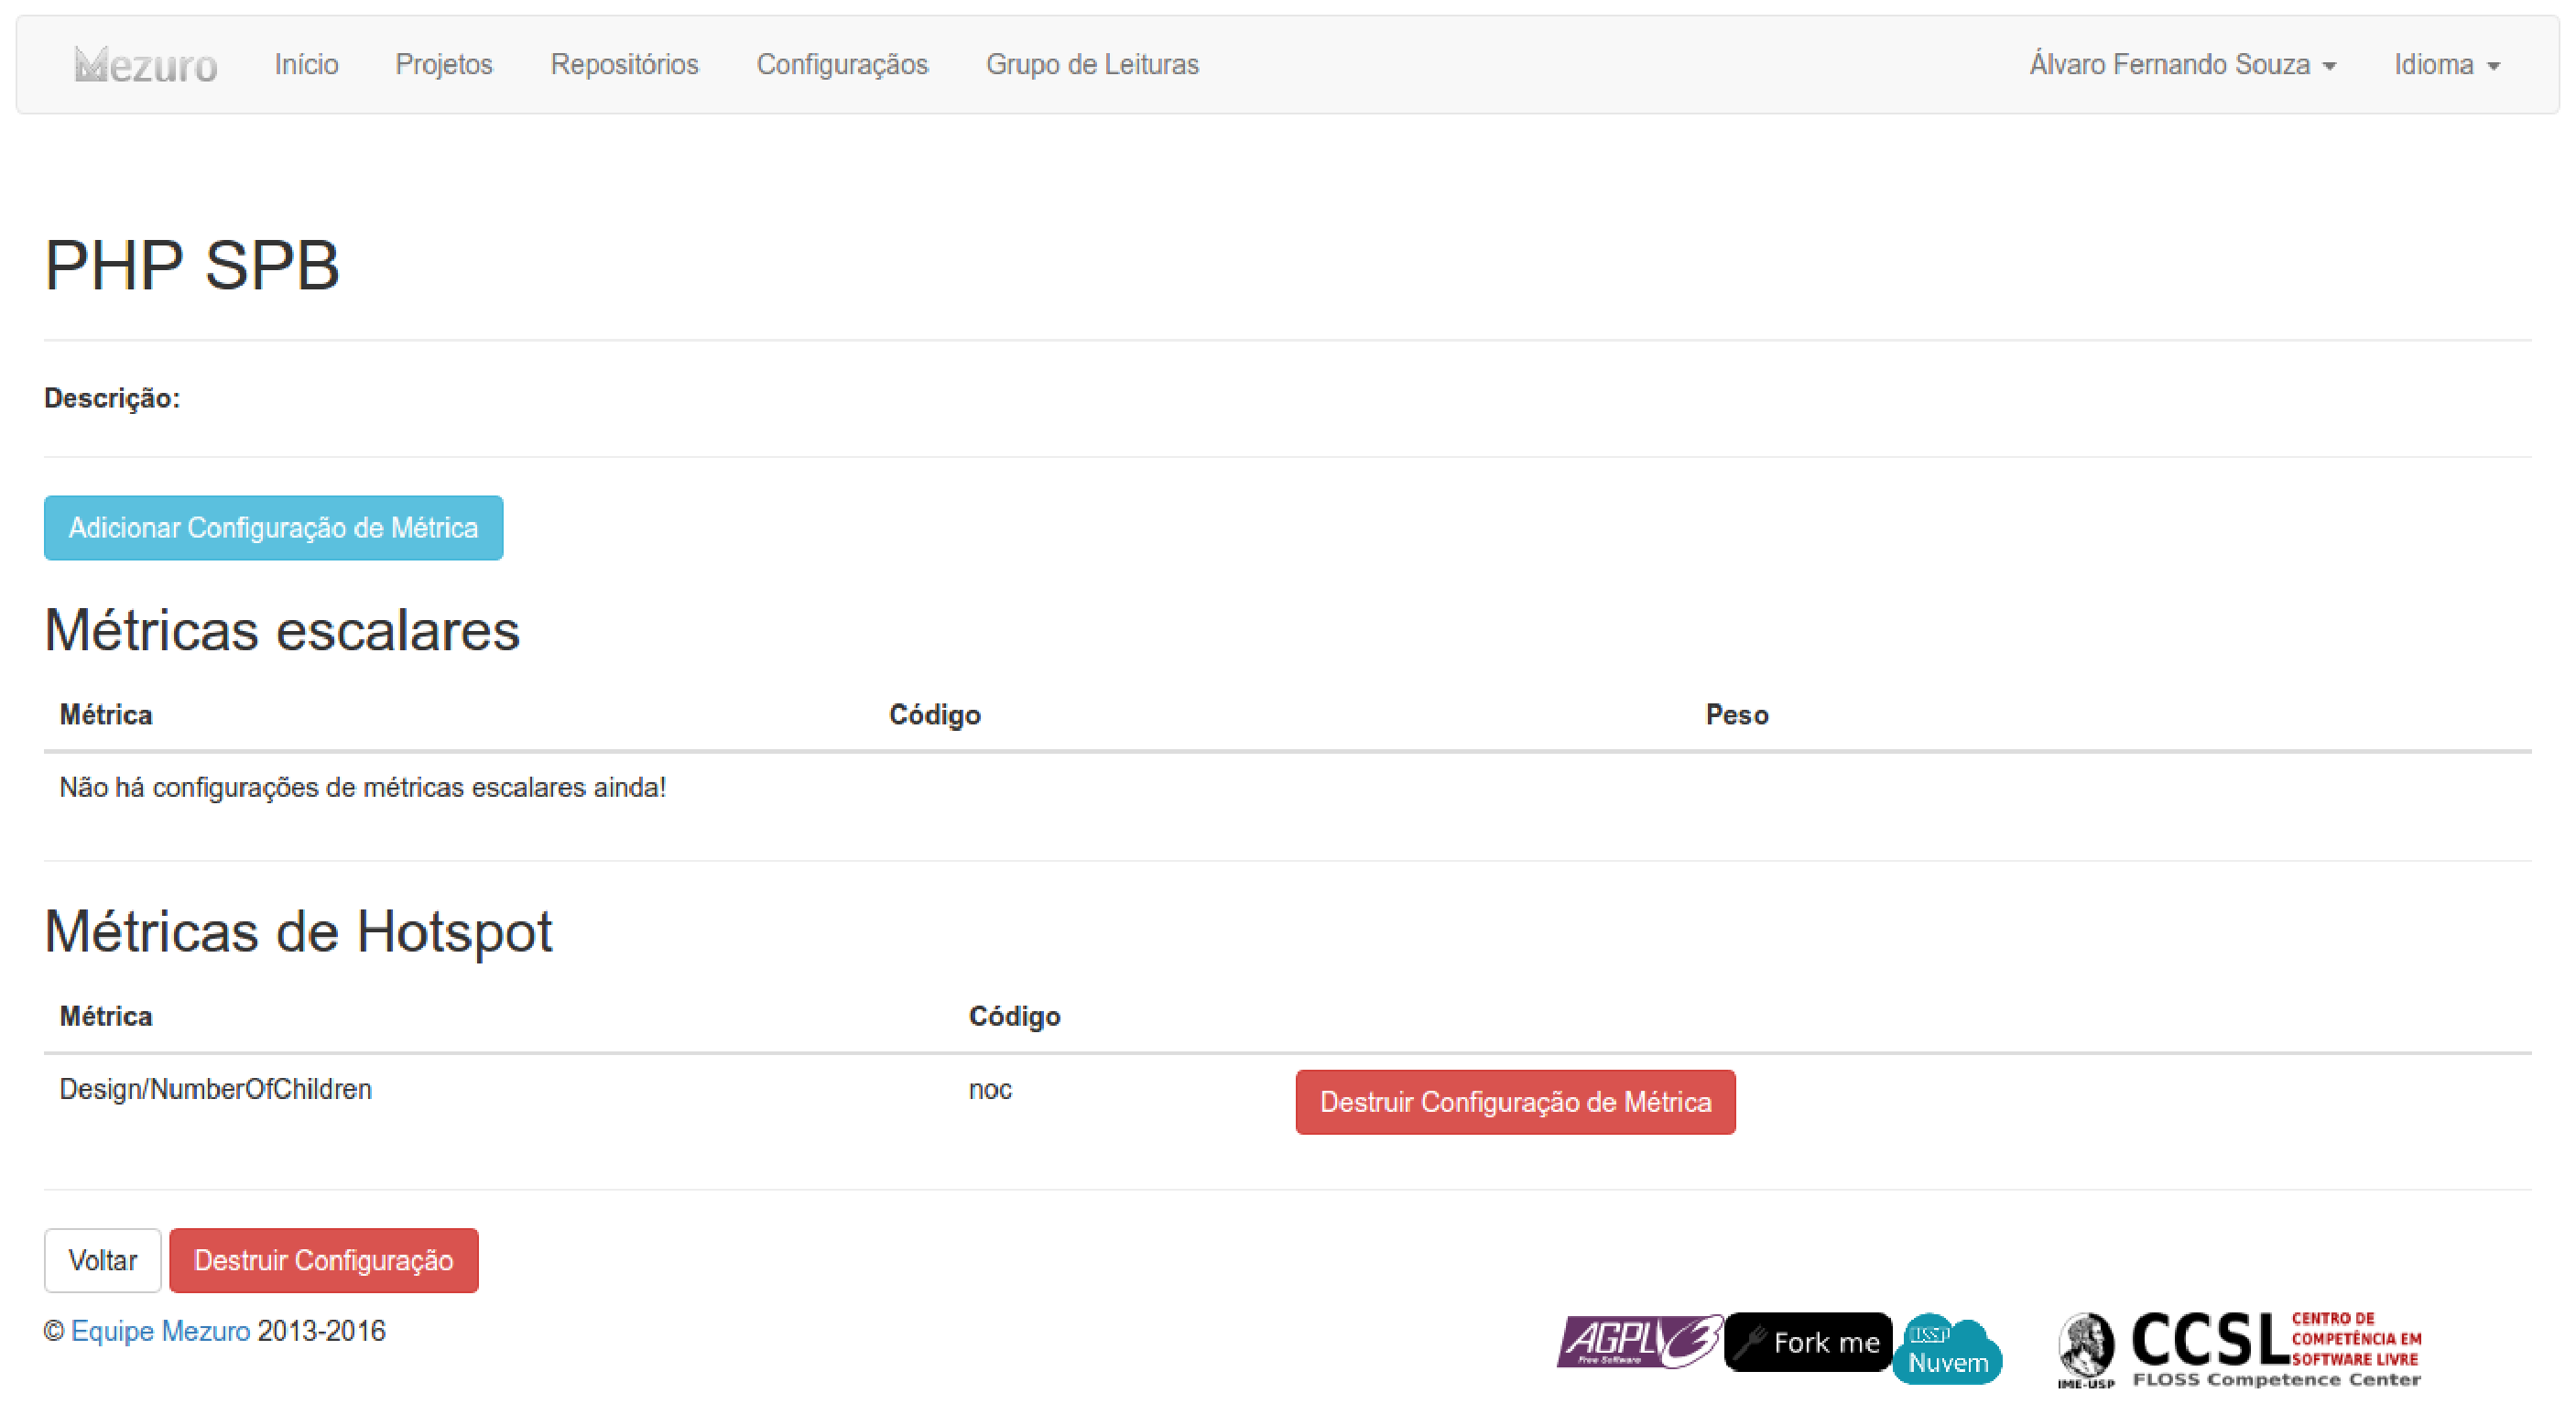
\includegraphics[keepaspectratio=true,scale=0.3]
    {figuras/mezuro-configuracao-view.eps}
  \caption{Mezuro - Página de Configuração}
	\label{fig:mezuro-configuracao-view}
\end{figure}

\begin{figure}[!htb]
	\centering
    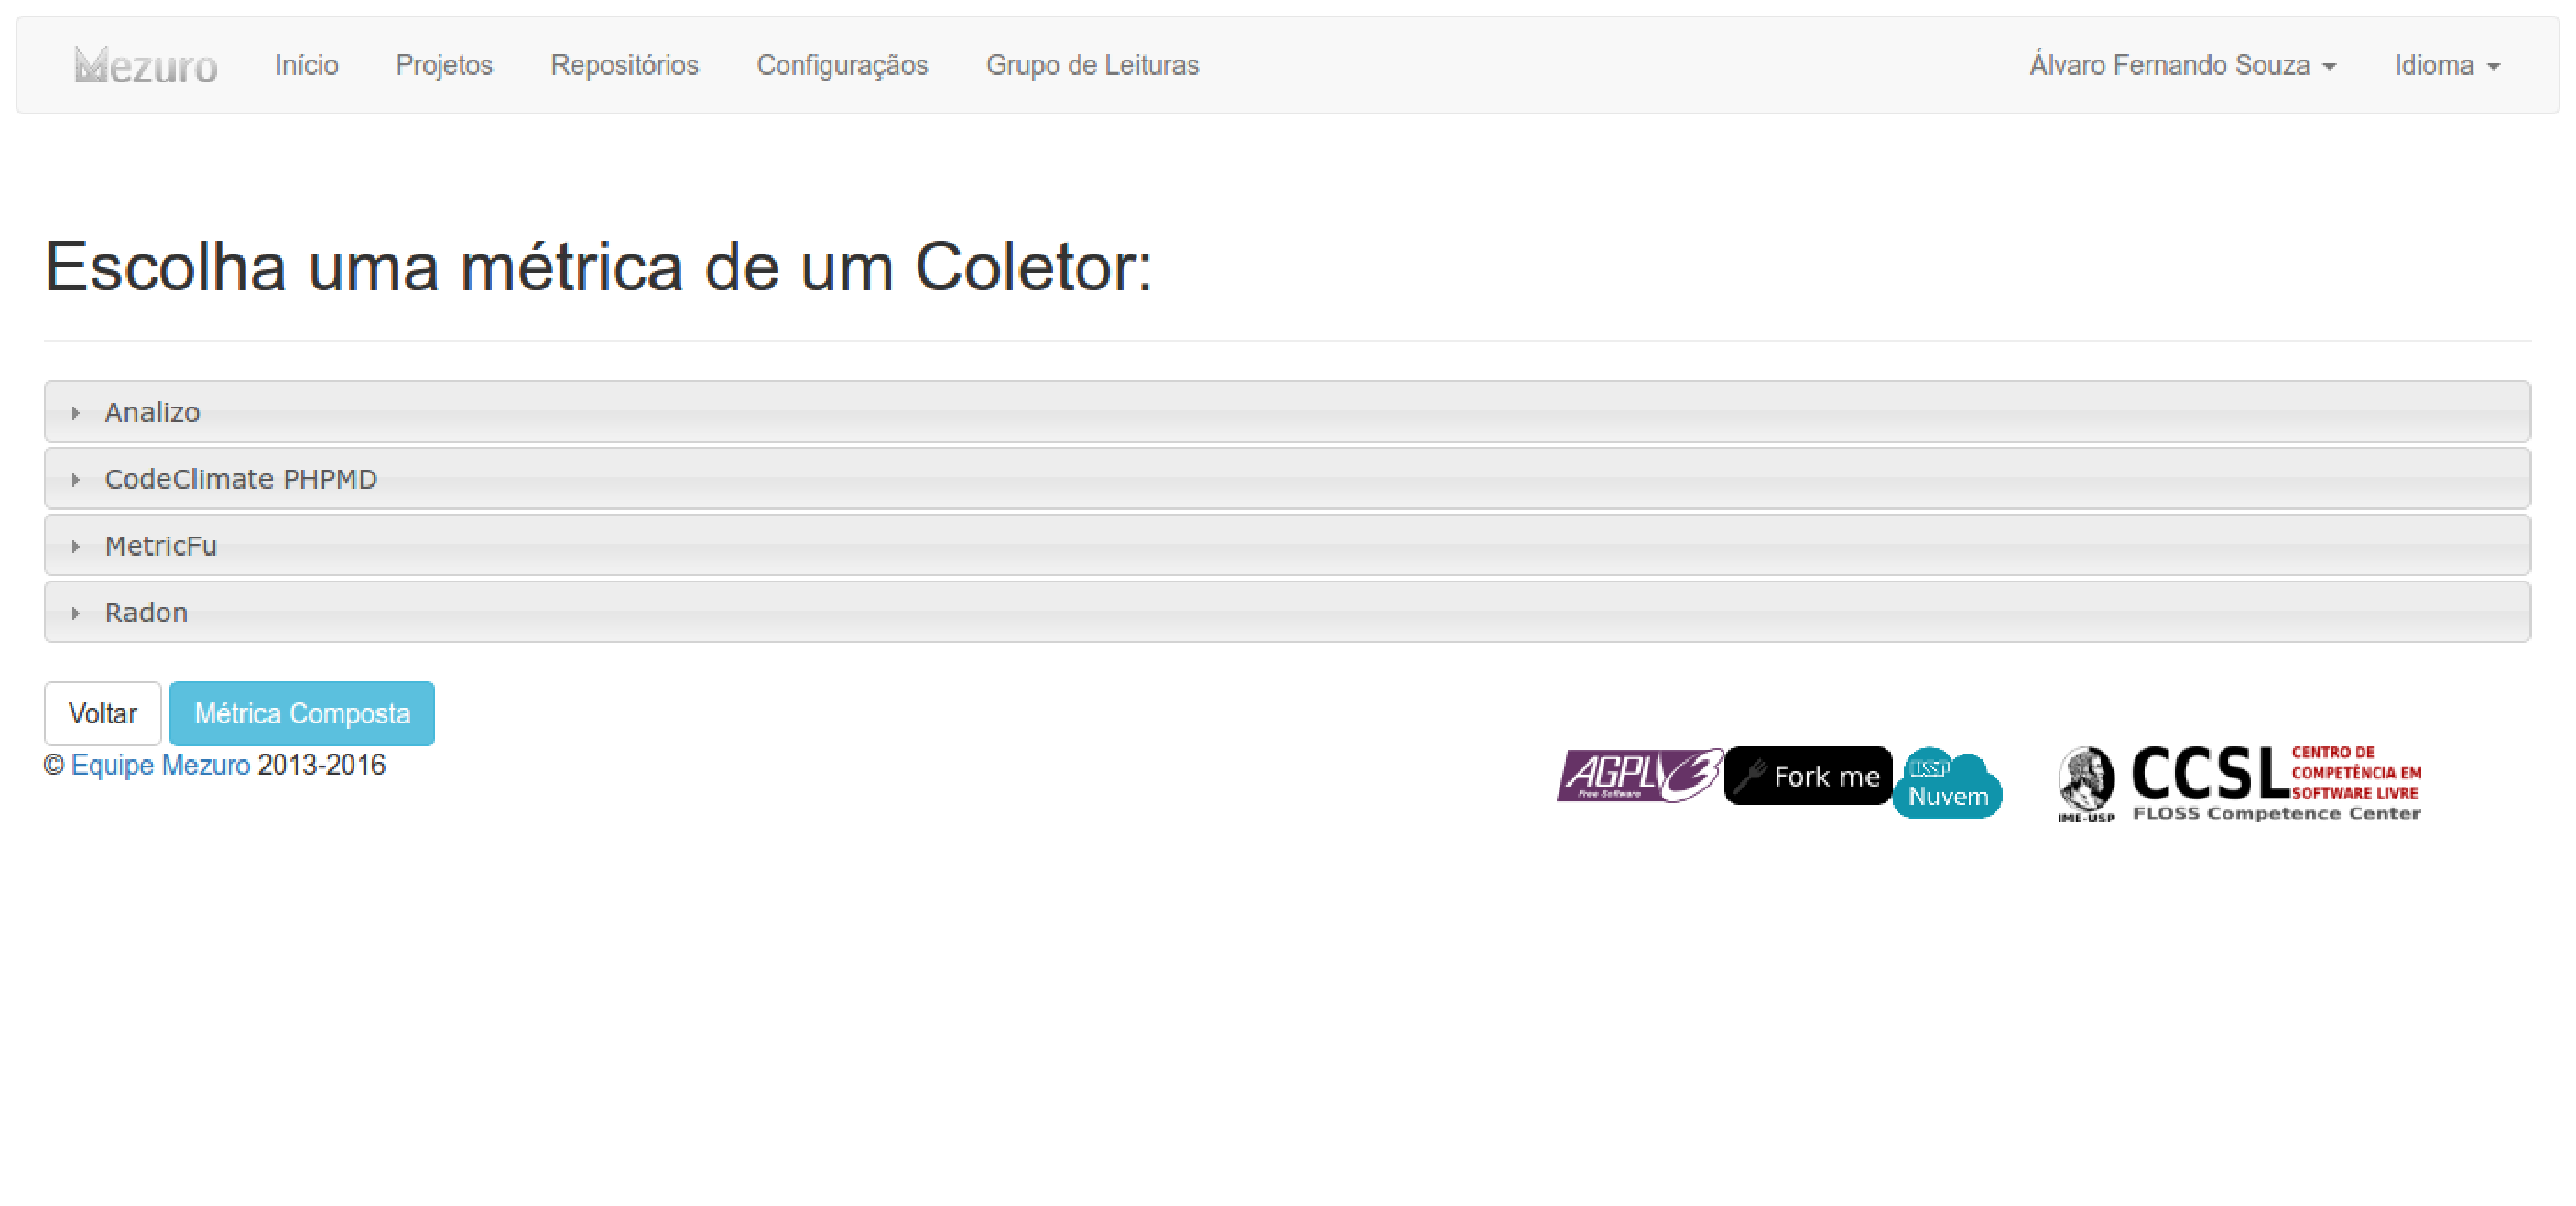
\includegraphics[keepaspectratio=true,scale=0.3]
    {figuras/mezuro-configuracao-add-metric.eps}
  \caption{Mezuro - Adicionar Métrica}
	\label{fig:mezuro-configuracao-add-metric}
\end{figure}

\newpage

Para a criação dos Grupos de Leitura, basta também, informar o nome e descrição.
E em seguida, adicionar um leitura, indicando o rótulo que se é desejado atribuir,
a nota, e uma cor.

\begin{figure}[!htb]
	\centering
    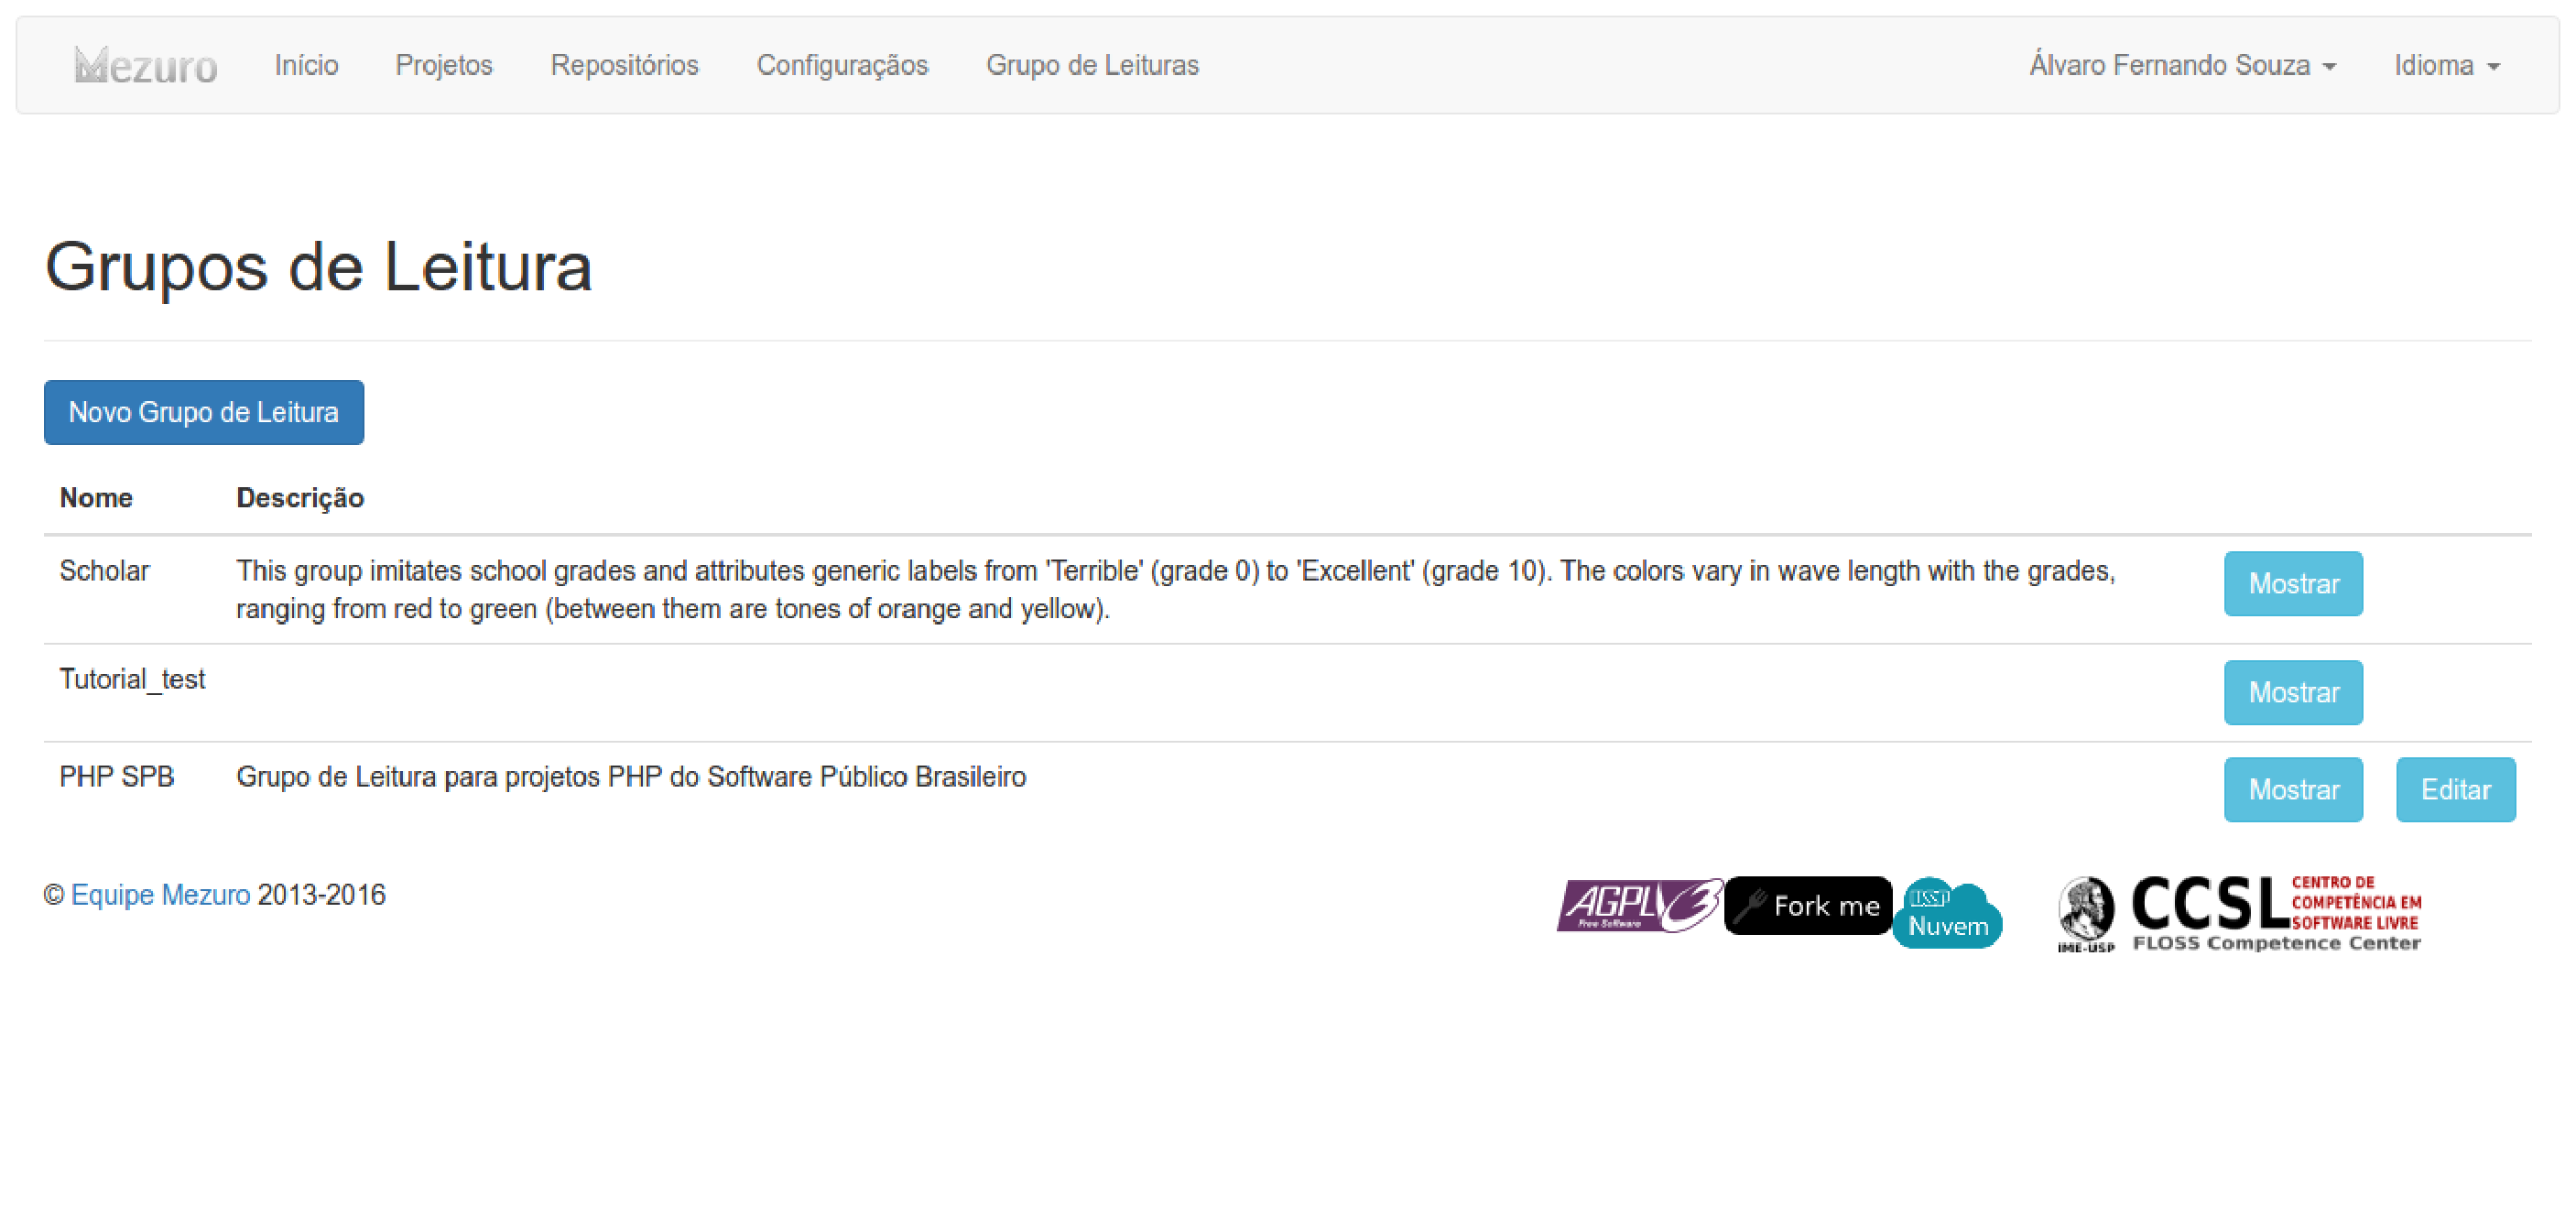
\includegraphics[keepaspectratio=true,scale=0.3]
    {figuras/mezuro-leituras.eps}
  \caption{Mezuro - Lista de Grupos de Leitura}
	\label{fig:mezuro-leituras}
\end{figure}

\begin{figure}[!htb]
	\centering
    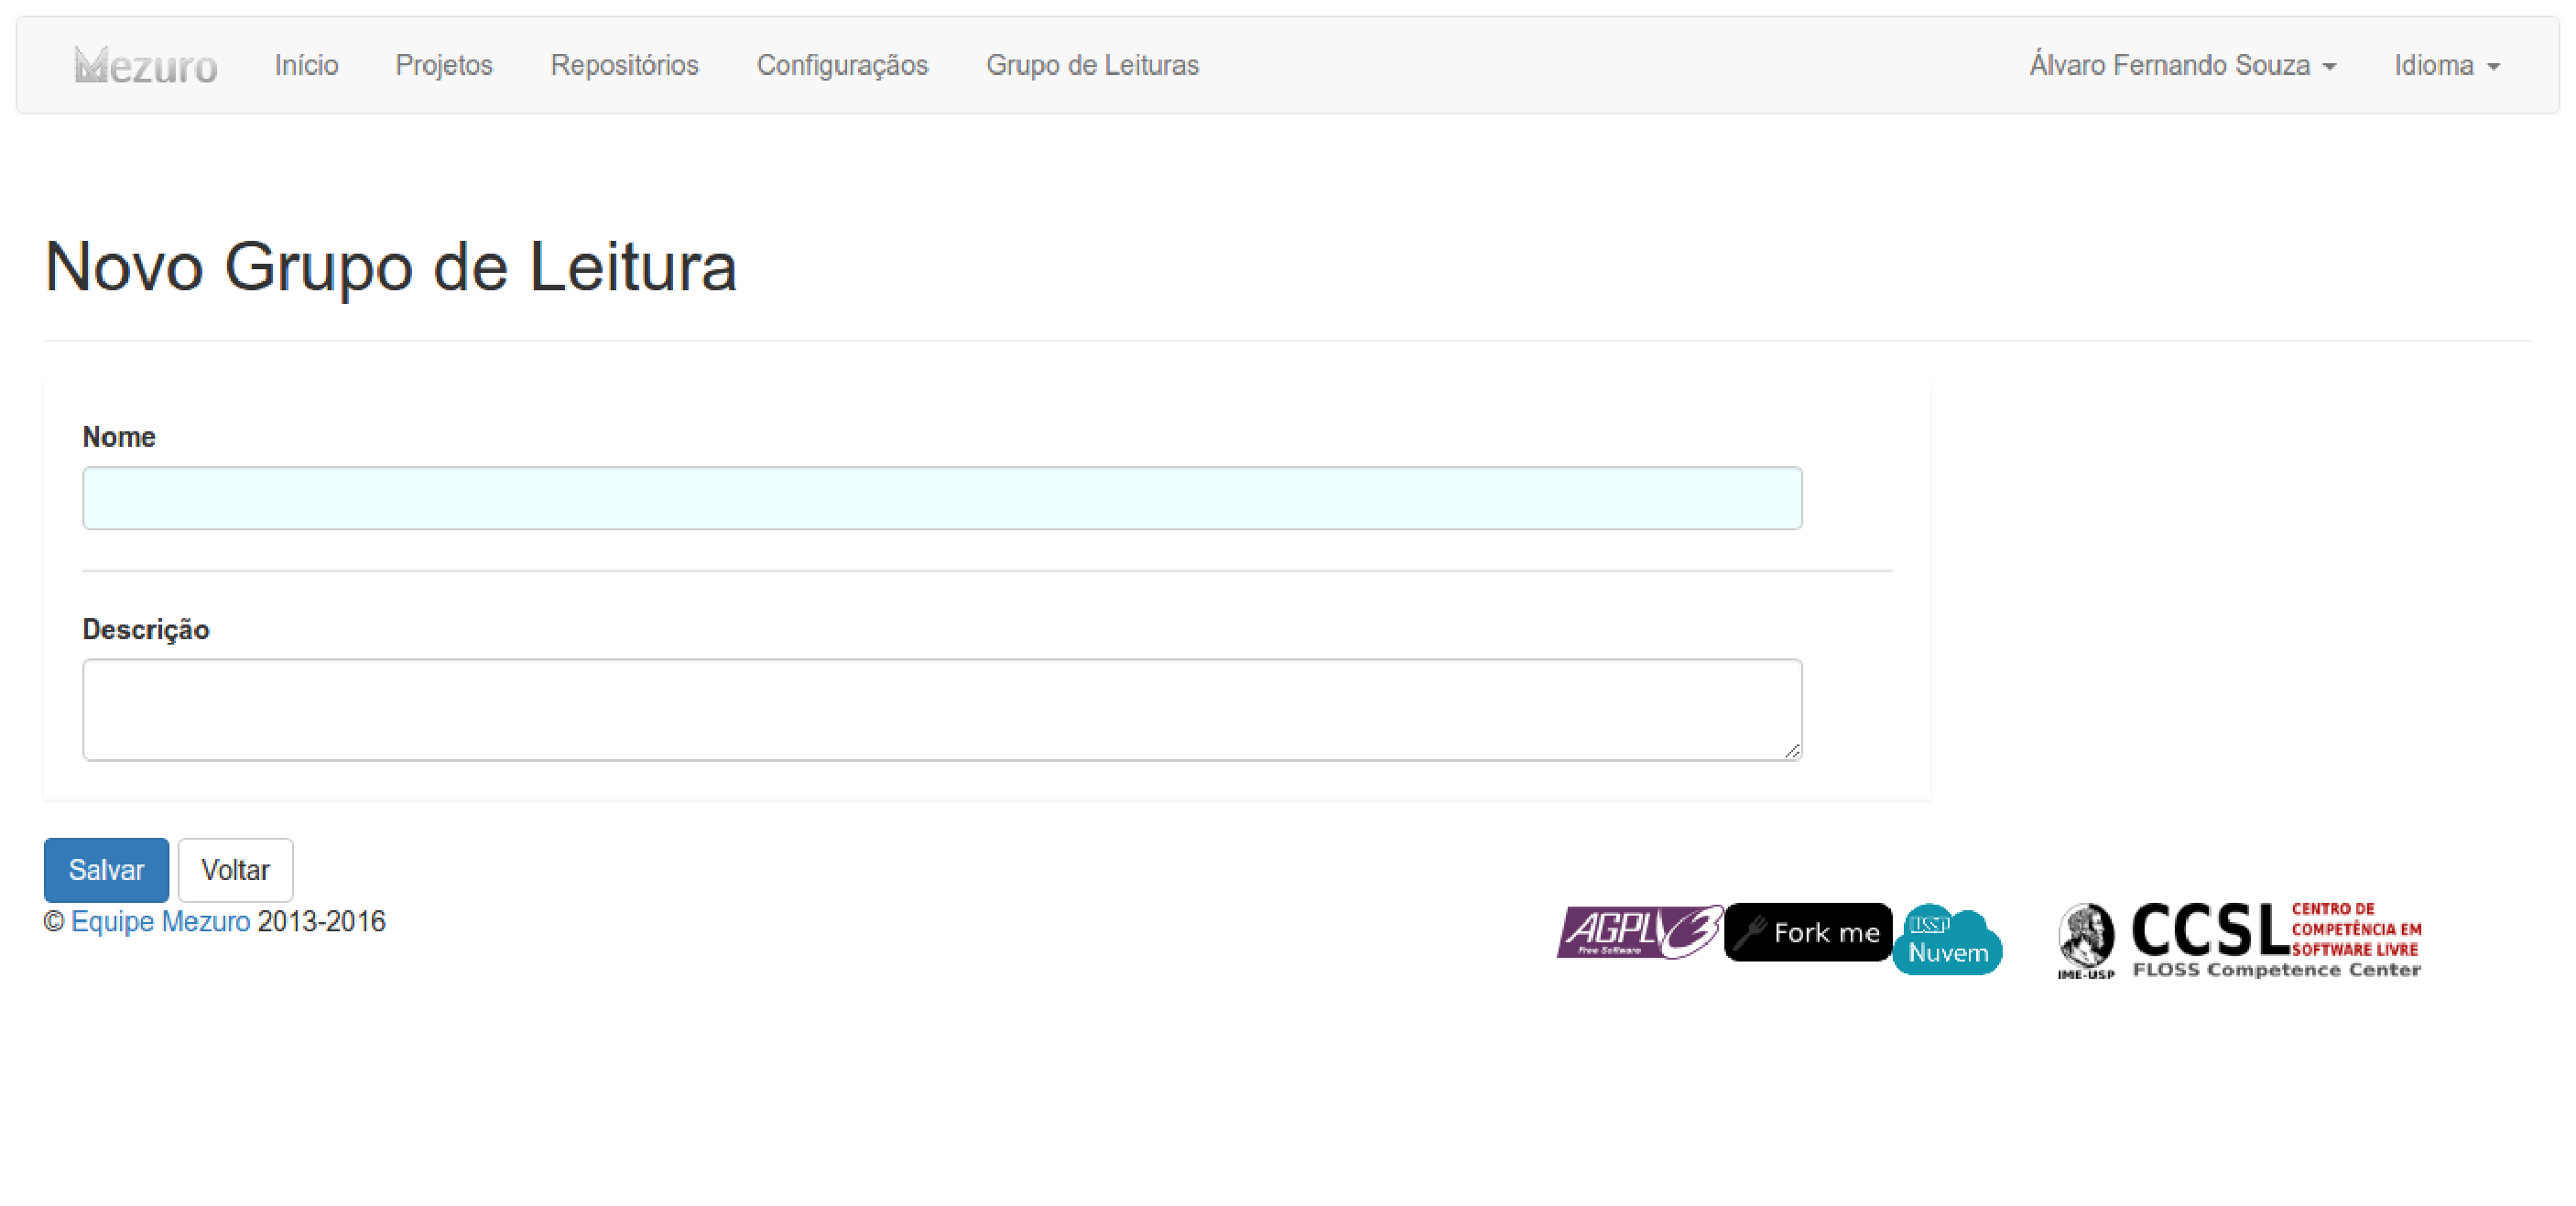
\includegraphics[keepaspectratio=true,scale=0.3]
    {figuras/mezuro-leitura-cadastro.eps}
  \caption{Mezuro - Cadastro de Grupos de Leitura}
	\label{fig:mezuro-leitura-cadastro}
\end{figure}

\newpage

\begin{figure}[!htb]
	\centering
    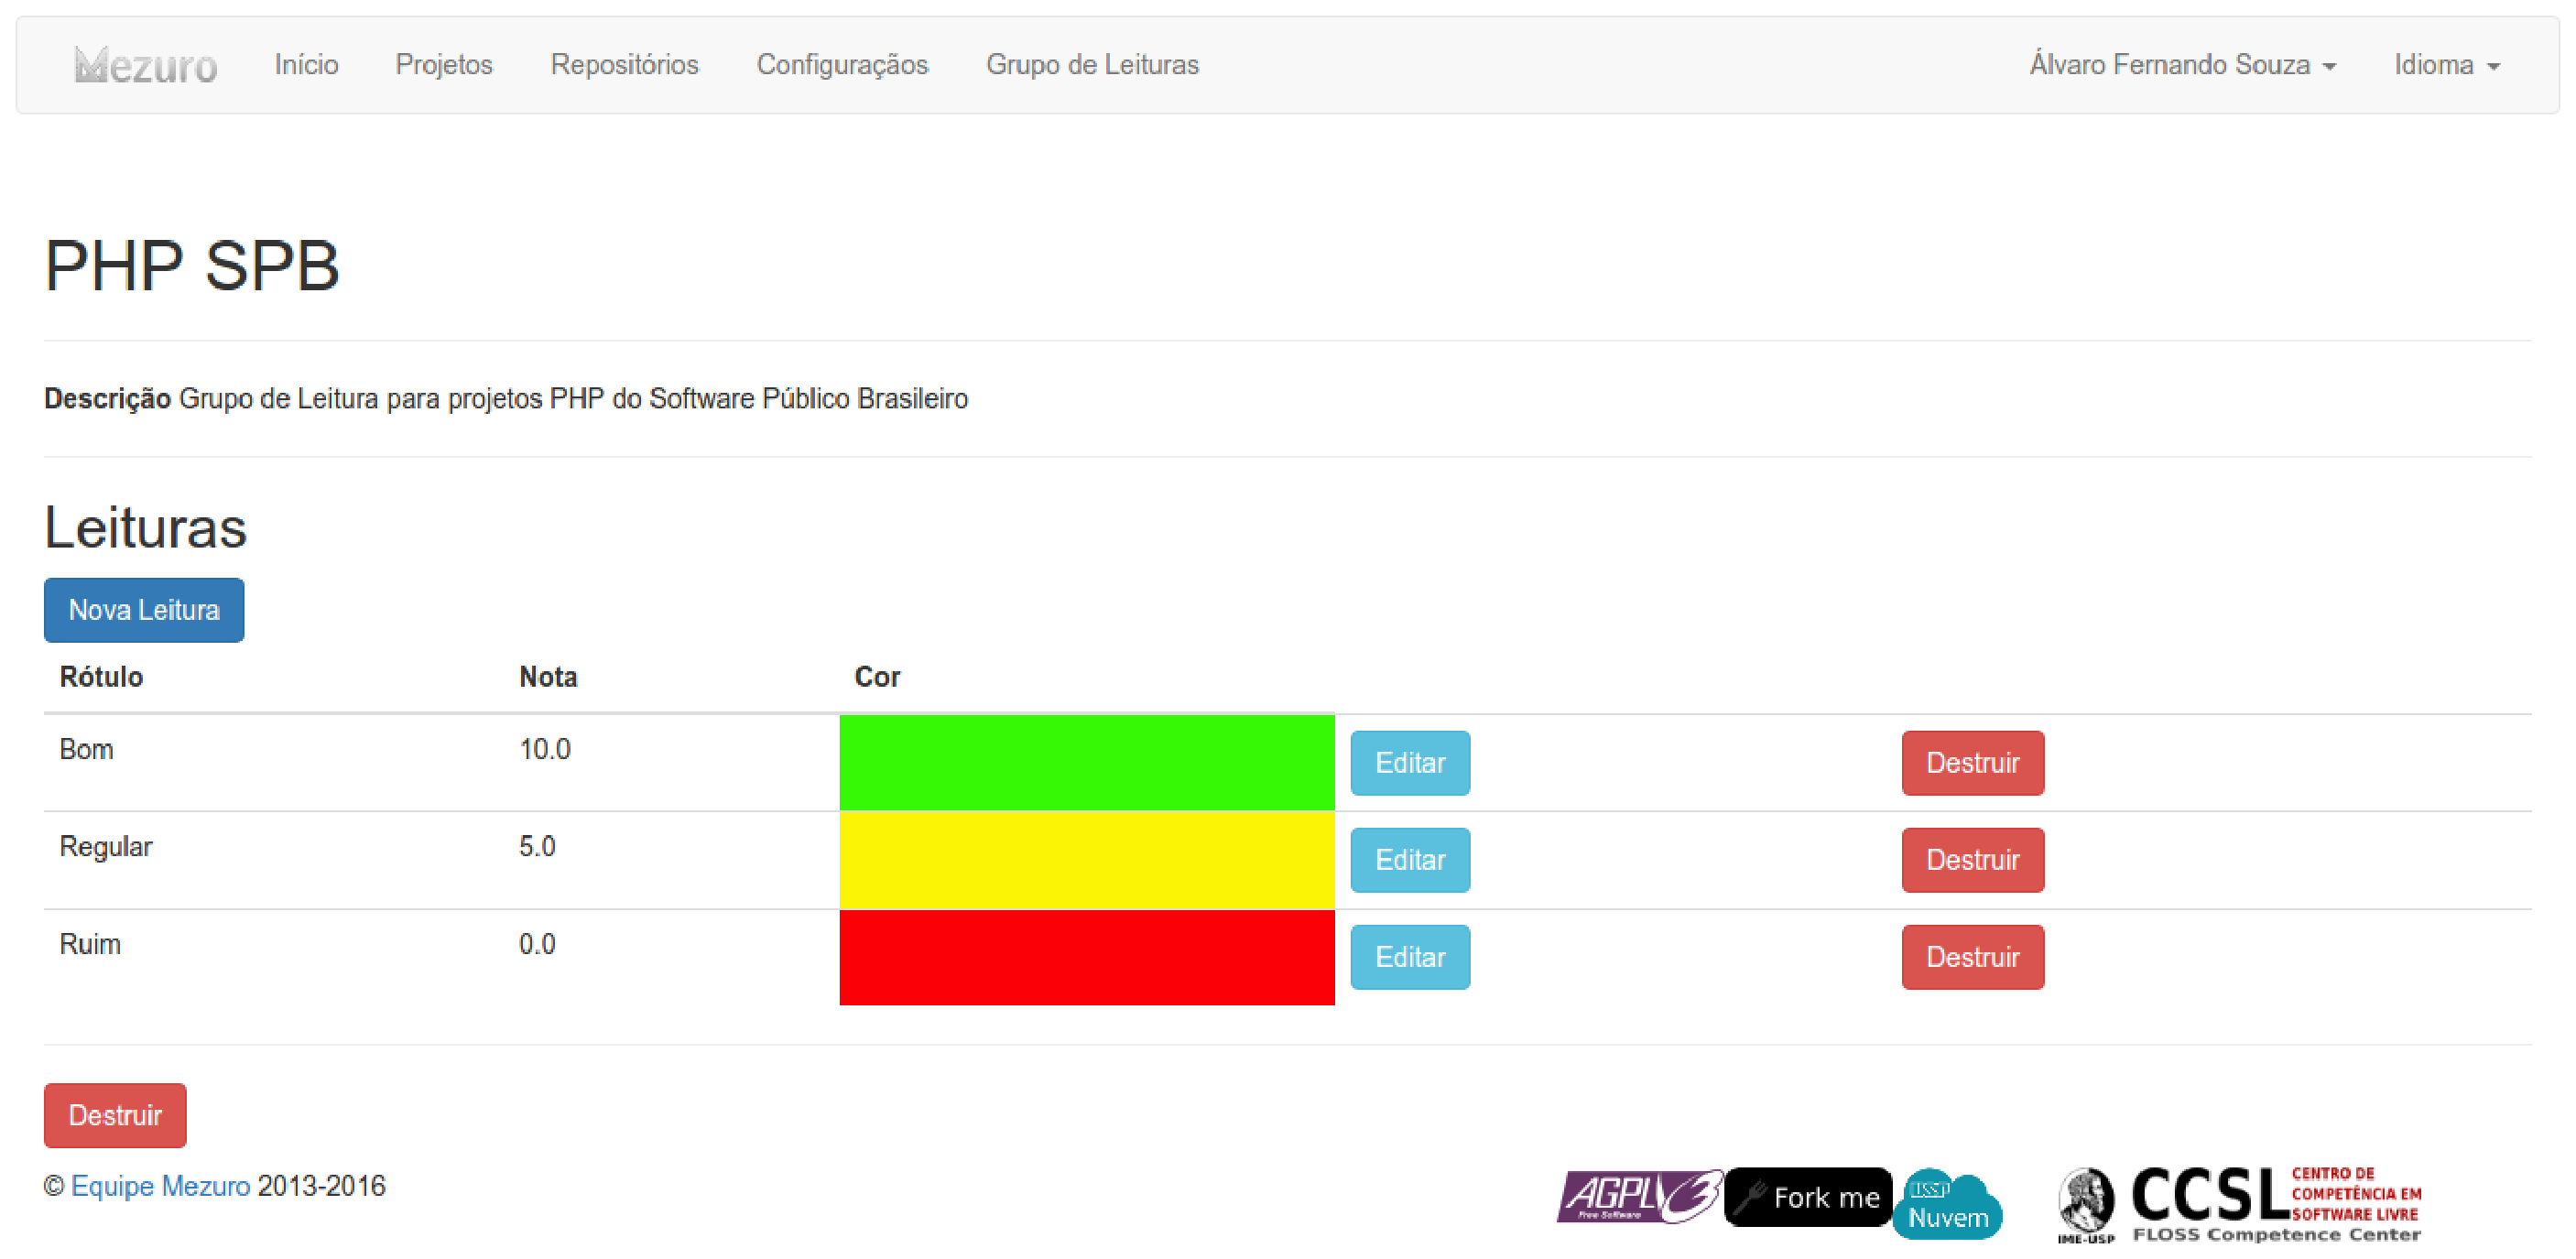
\includegraphics[keepaspectratio=true,scale=0.3]
    {figuras/mezuro-leitura-view.eps}
  \caption{Mezuro - Página de um Grupo de Leitura}
	\label{fig:mezuro-leitura-view}
\end{figure}

\begin{figure}[!htb]
	\centering
    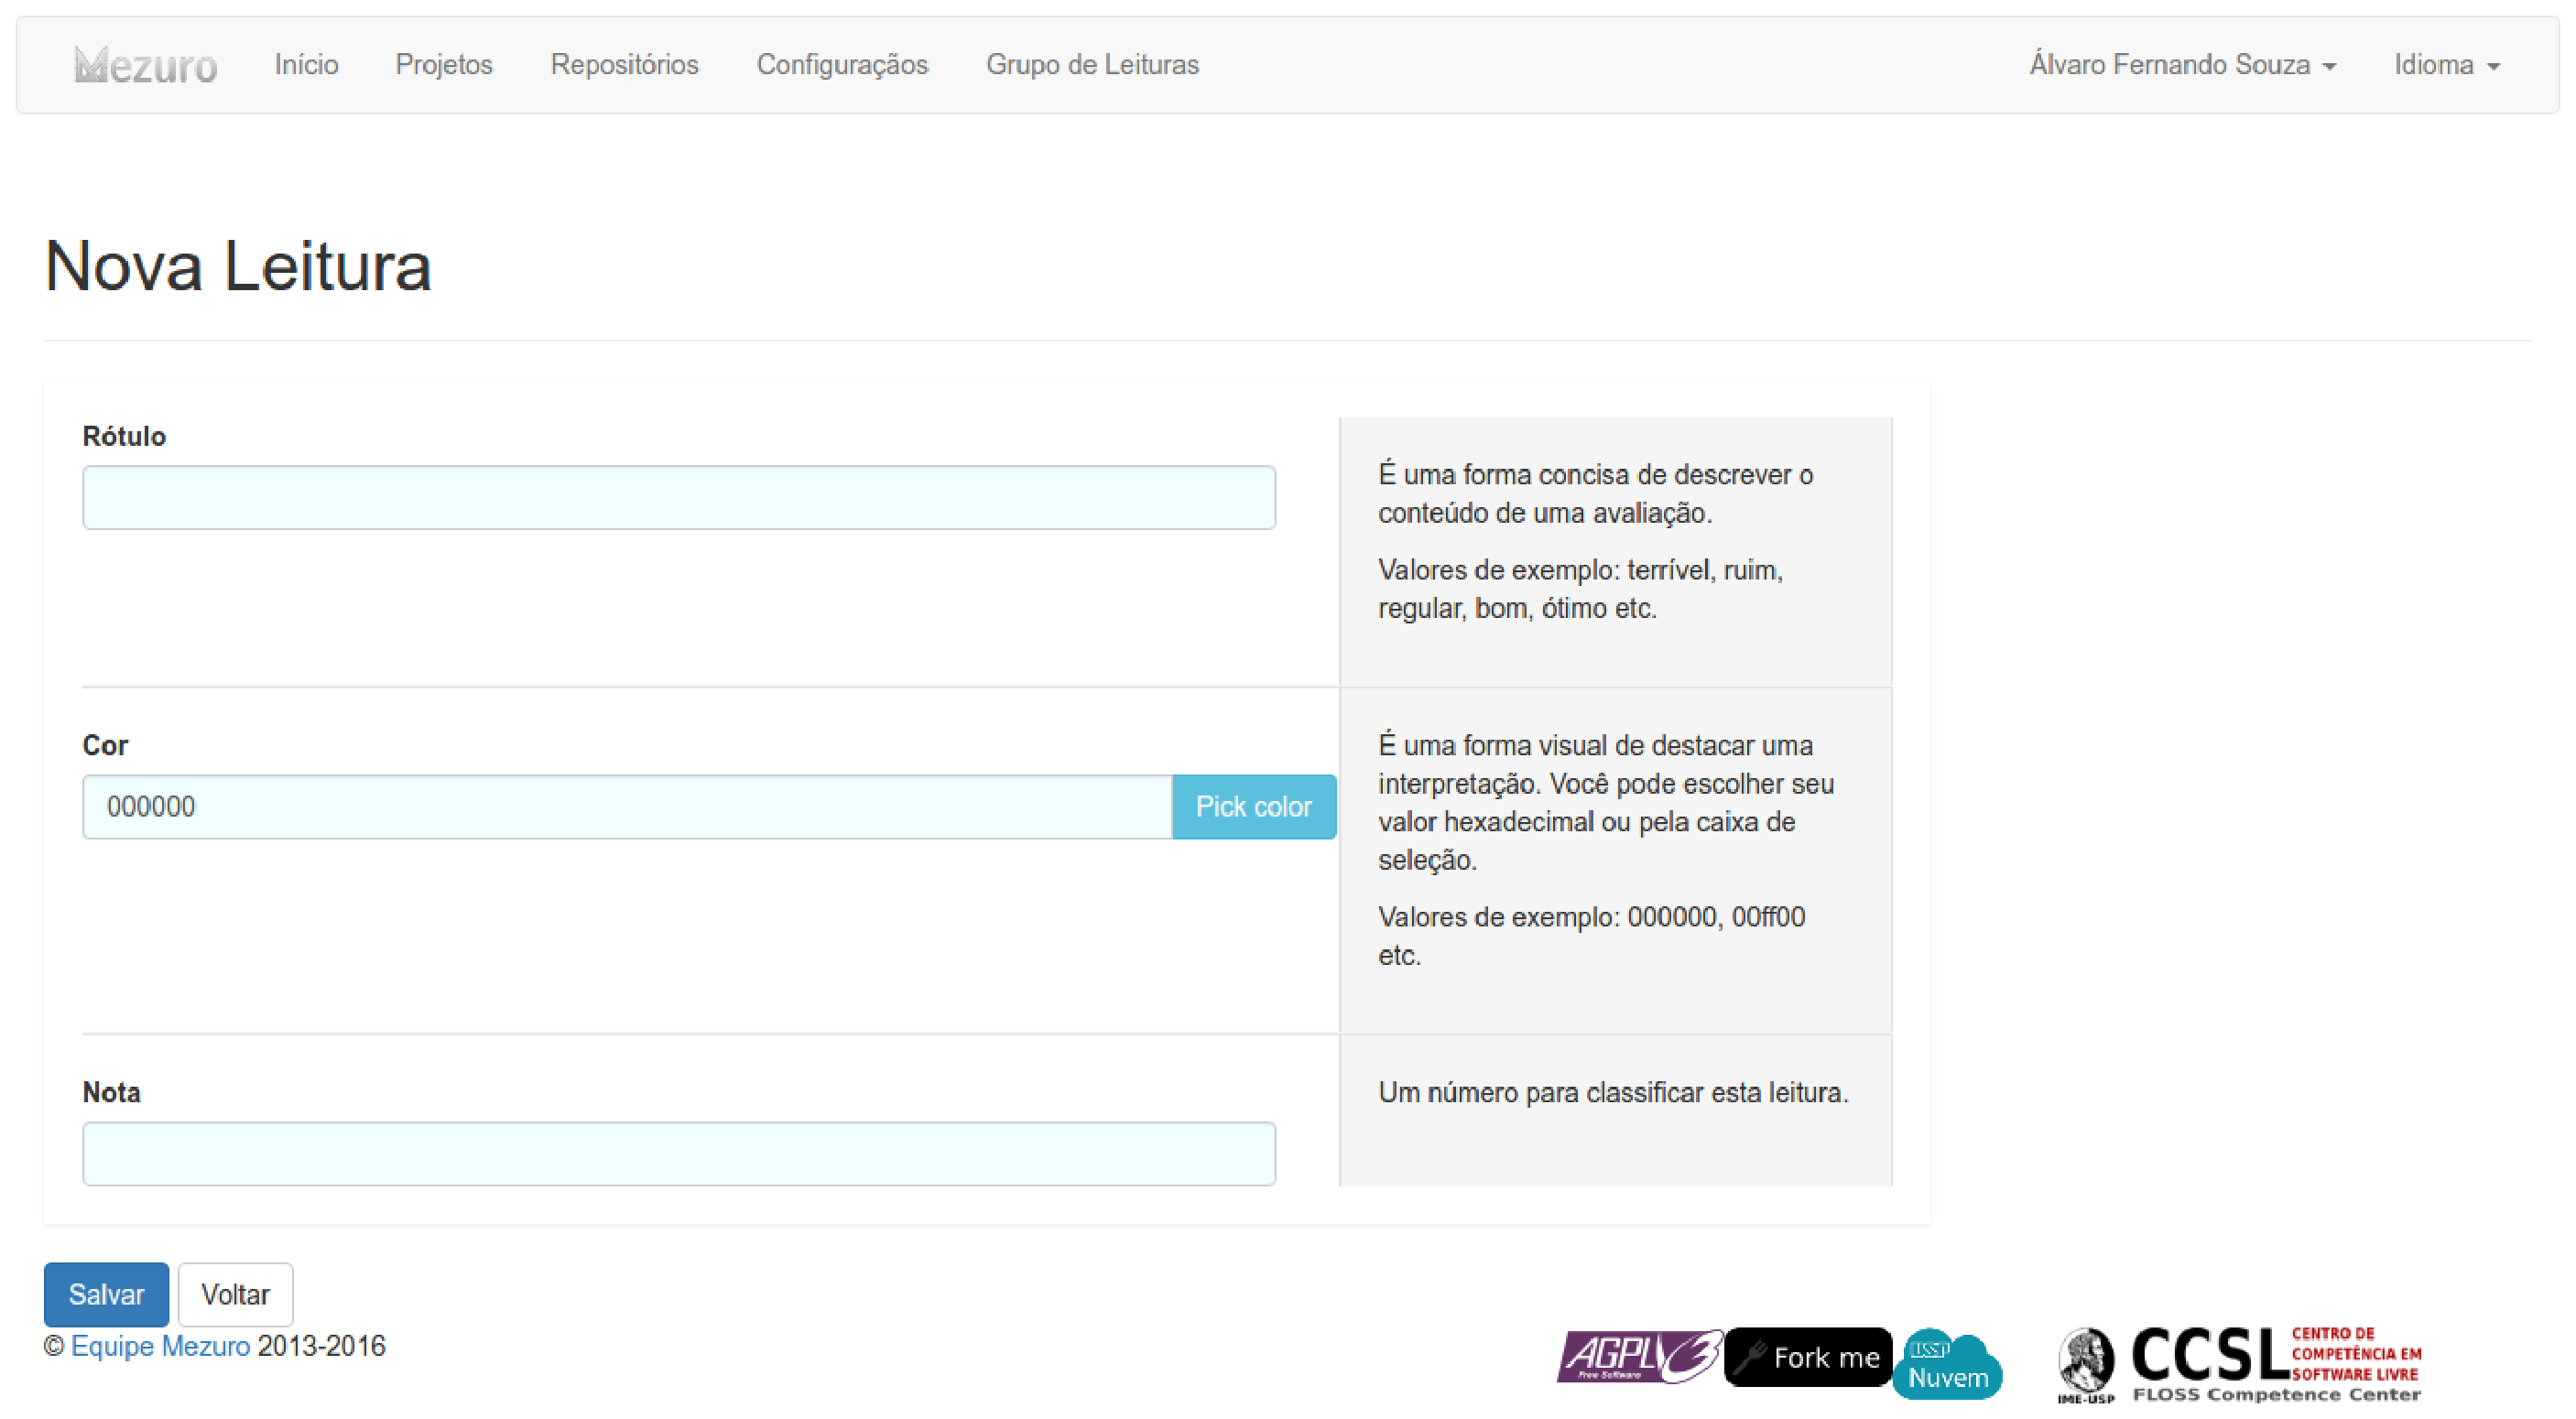
\includegraphics[keepaspectratio=true,scale=0.3]
    {figuras/mezuro-leitura-add.eps}
  \caption{Mezuro - Adicionar Leitura}
	\label{fig:mezuro-leitura-add}
\end{figure}

\newpage

A página de exibição dos resultados da avaliação é composta por informações do
repositório, do processamento, árvore de módulos, resultados de métricas de
\textit{hotspot} e resultados de métrica. A Figura \ref{fig:mezuro-repositorio-view}
mostra os resultados da análise\footnote{\url{http://mezuro.org/pt/repositories/114}}
de um dos softwares do SPB, o Xemelê
\footnote{\url{https://softwarepublico.gov.br/social/xemele}}.
As métricas são expotas por conjuntos de resultados: métricas \textit{hotspot} e
demais métricas. Na opção de ``Árvore de Módulos'', é possível navegar nos
diretórios do projeto e verificar os resultados para determinada camada do
sistema. Por exemplo: caso o usuário queira visualizar as métricas da classe
\textit{xpto}, que está no diretório \textit{app/model/}, ele precisa ir
clicando na árvore de diretórios do projeto até chegar no desejado.

\begin{figure}[!htb]
	\centering
    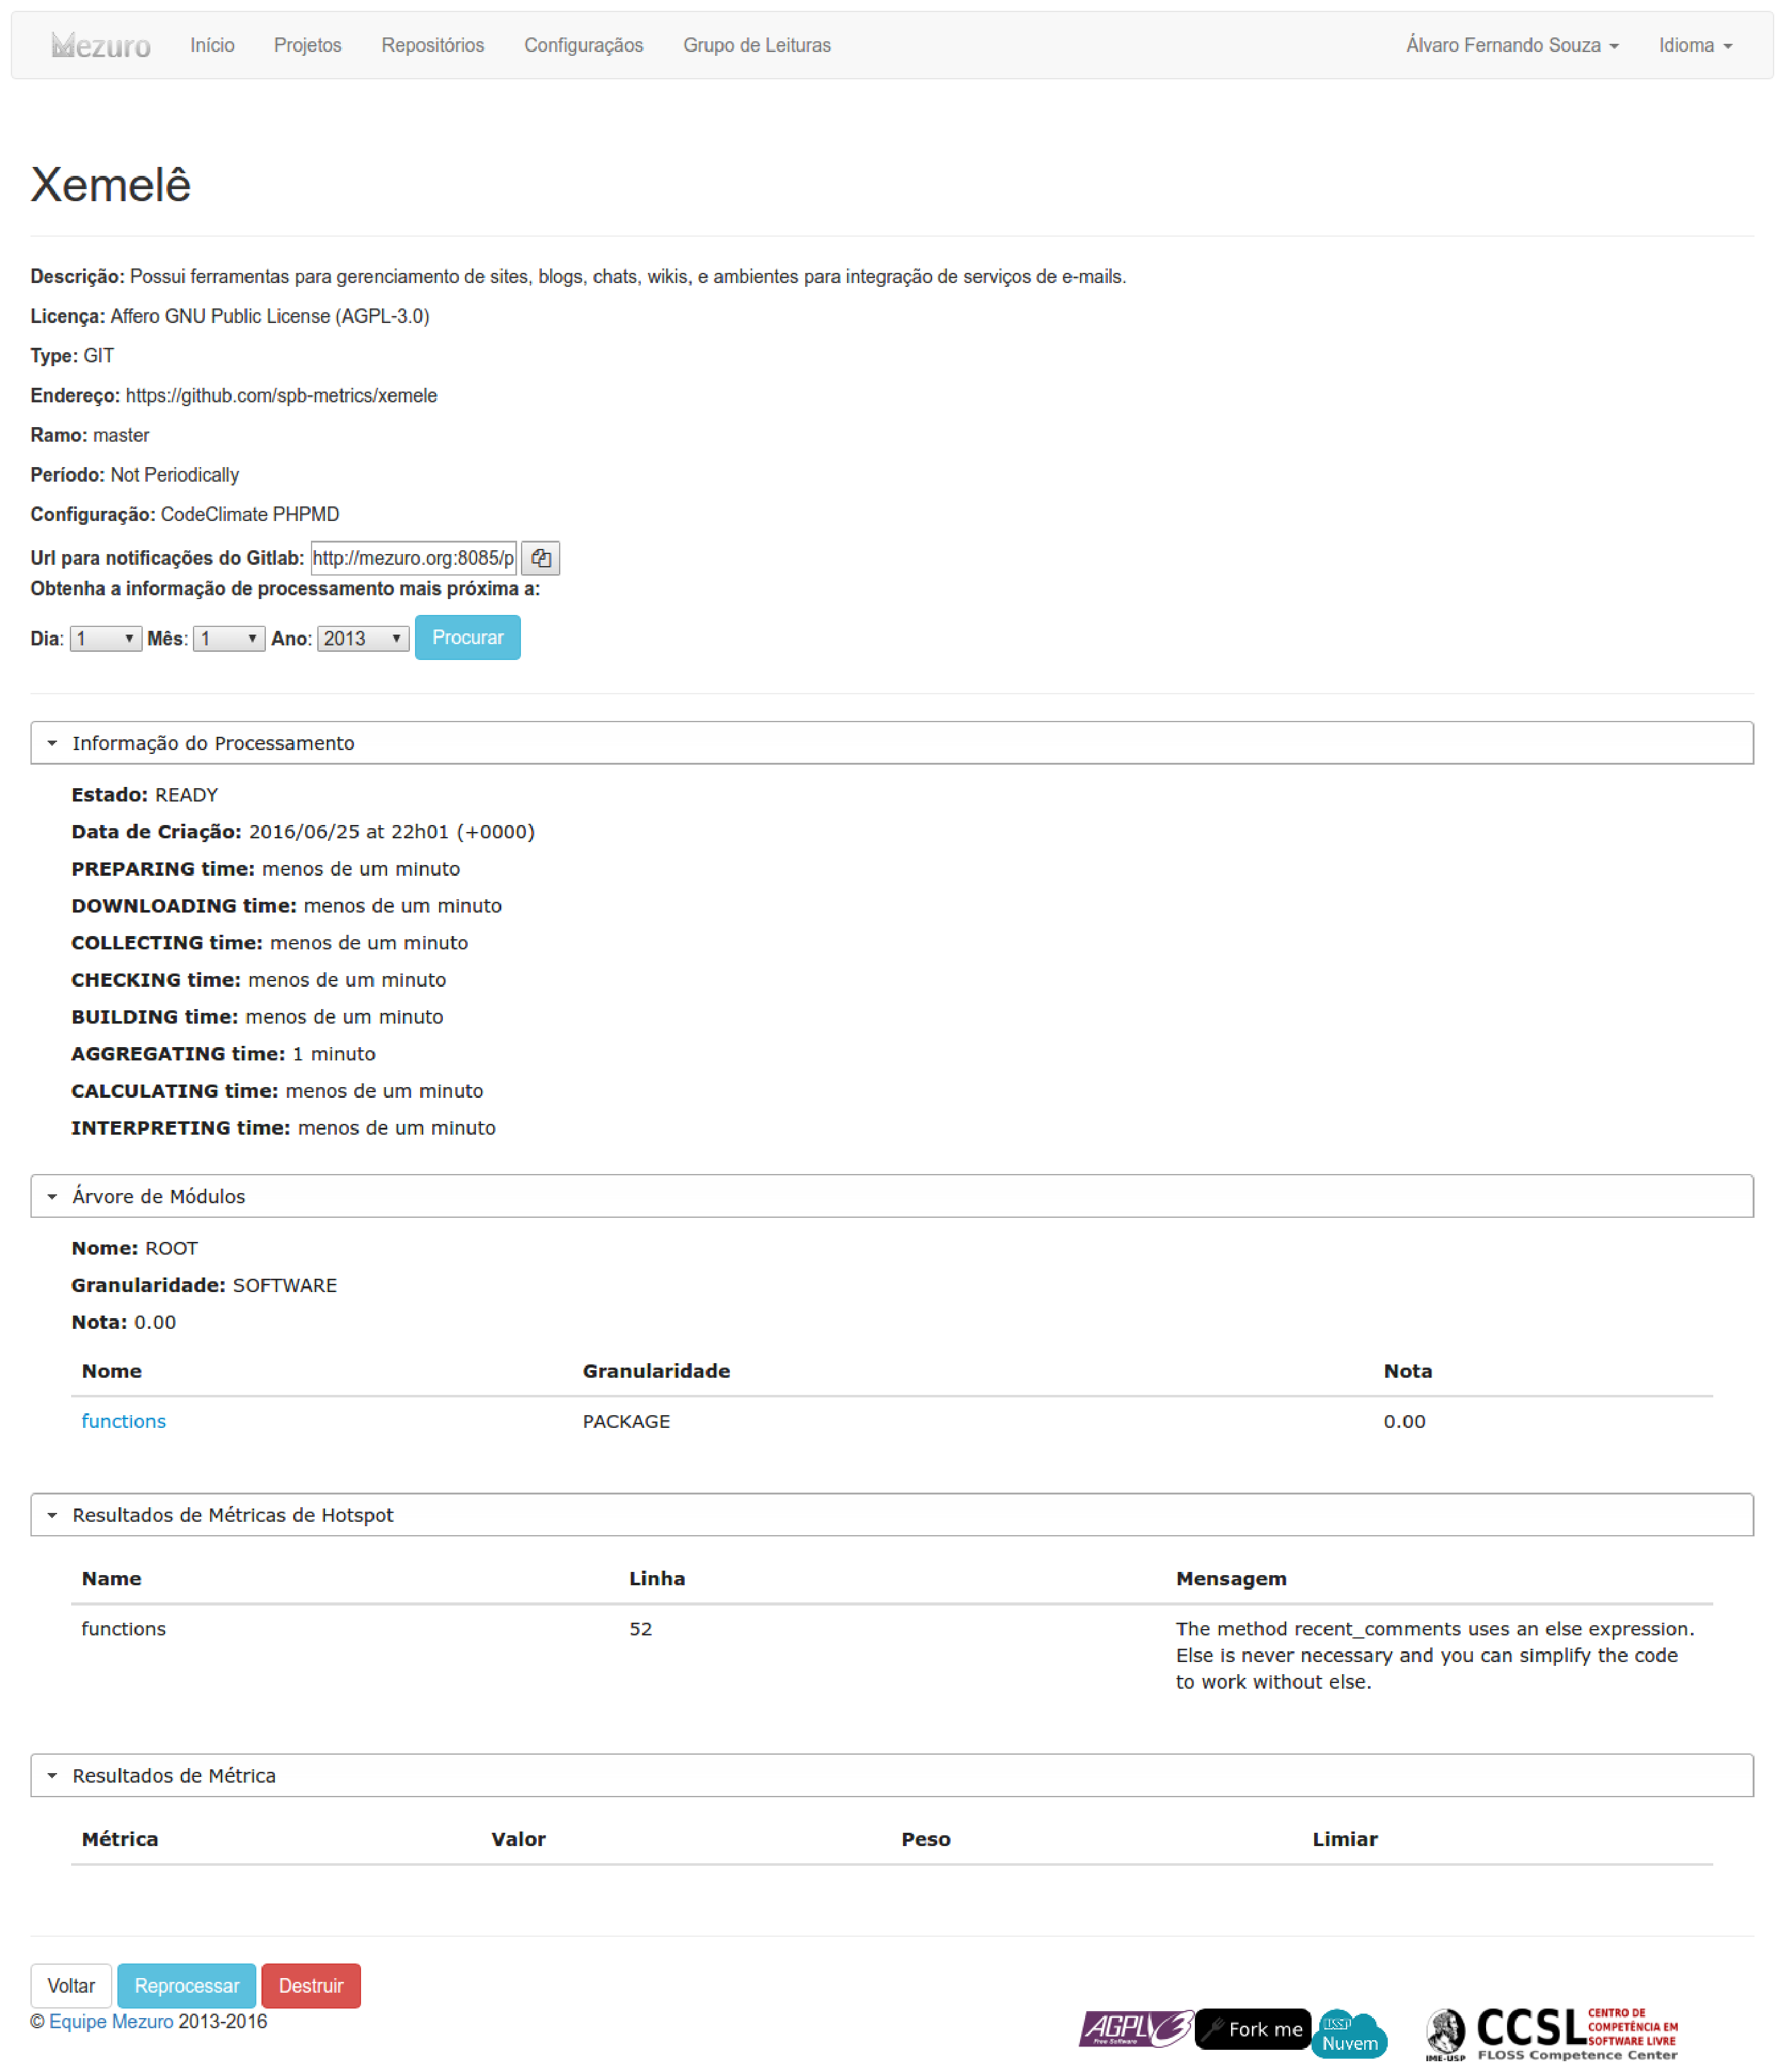
\includegraphics[keepaspectratio=true,scale=0.3]
    {figuras/mezuro-repositorio-view.eps}
  \caption{Mezuro - Página de Repositório}
	\label{fig:mezuro-repositorio-view}
\end{figure}
